% Seminarul 2: Modele ARMA
% Serii de timp -- Programele de licență Informatică economică și Cibernetică economică, Academia de Studii Economice din București
% GENERAT de latex/build_seminar2.py -- modificați generatorul, nu acest fișier.
% Implicit versiunea pentru studenți; versiunea profesorului este wrapper-ul *_solutions.tex.
\makeatletter\@ifundefined{ifsolutions}{\expandafter\newif\csname ifsolutions\endcsname}{}\makeatother

\newcommand{\coursename}{Serii de timp}
\def\tsalang{ro}
% Preambul comun TSA -- Serii de timp / Time Series Analysis (Beamer, 16:9)
% Același design ca MFM și SFM (preluat din SFM, 5 octombrie 2026). Înainte de % Preambul comun TSA -- Serii de timp / Time Series Analysis (Beamer, 16:9)
% Același design ca MFM și SFM (preluat din SFM, 5 octombrie 2026). Înainte de % Preambul comun TSA -- Serii de timp / Time Series Analysis (Beamer, 16:9)
% Același design ca MFM și SFM (preluat din SFM, 5 octombrie 2026). Înainte de \input{../../latex/preamble} se definește
%   \newcommand{\coursename}{Time Series Analysis}      (EN)
%   \newcommand{\coursename}{Serii de timp}       (RO)  și  \def\tsalang{ro}
% Fișierele .tex se află în EN/Courses, EN/Seminars, RO/Cursuri, RO/Seminarii (două niveluri sub rădăcină).
% Deck-urile sînt generate de latex/build_chapterN.py / build_seminarN.py (vezi latex/tsa_build.py).

\documentclass[9pt, aspectratio=169, t]{beamer}
\providecommand{\coursename}{Time Series Analysis}

% Ensure content fits on slides
\setbeamersize{text margin left=8mm, text margin right=8mm}
% Smaller institute font (title page)
\setbeamerfont{institute}{size=\footnotesize}

%=============================================================================
% THEME AND STYLE CONFIGURATION
%=============================================================================
\usetheme{default}
% Using default theme for clean header/footer control

% Color Palette (matching Redispatch PDF)
\definecolor{MainBlue}{RGB}{26, 58, 110}
\definecolor{AccentBlue}{RGB}{26, 58, 110}
\definecolor{IDAred}{RGB}{205, 0, 0}
\definecolor{DarkGray}{RGB}{51, 51, 51}
\definecolor{MediumGray}{RGB}{128, 128, 128}
\definecolor{LightGray}{RGB}{248, 248, 248}
\definecolor{VeryLightGray}{RGB}{235, 235, 235}
\definecolor{KeynoteGray}{RGB}{218, 218, 218}
\definecolor{SectionGray}{RGB}{120, 120, 120}
\definecolor{FooterGray}{RGB}{100, 100, 100}
\definecolor{Crimson}{RGB}{220, 53, 69}
\definecolor{Forest}{RGB}{46, 125, 50}
\definecolor{Amber}{RGB}{181, 133, 63}
\definecolor{Orange}{RGB}{230, 126, 34}
\definecolor{Purple}{RGB}{142, 68, 173}

% Gradient background (exact Keynote 315° gradient: white to RGB 218,218,218)
\setbeamertemplate{background}{%
    \begin{tikzpicture}[remember picture, overlay]
        \shade[shading=axis, shading angle=315,
        top color=white, bottom color=KeynoteGray]
        (current page.south west) rectangle (current page.north east);
    \end{tikzpicture}%
}
% Fallback solid color for compatibility
\setbeamercolor{background canvas}{bg=}

\setbeamercolor{palette primary}{bg=MainBlue, fg=white}
\setbeamercolor{palette secondary}{bg=MainBlue!85, fg=white}
\setbeamercolor{palette tertiary}{bg=MainBlue!70, fg=white}
\setbeamercolor{structure}{fg=MainBlue}
\setbeamercolor{title}{fg=IDAred}
\setbeamercolor{frametitle}{fg=IDAred, bg=}
\setbeamercolor{block title}{bg=MainBlue, fg=white}
\setbeamercolor{block body}{bg=VeryLightGray, fg=DarkGray}
\setbeamercolor{block title alerted}{bg=Crimson, fg=white}
\setbeamercolor{block body alerted}{bg=Crimson!8, fg=DarkGray}
\setbeamercolor{block title example}{bg=Forest, fg=white}
\setbeamercolor{block body example}{bg=Forest!8, fg=DarkGray}
\setbeamercolor{item}{fg=MainBlue}

% Footer colors (override Madrid theme blue)
\setbeamercolor{author in head/foot}{fg=FooterGray, bg=}
\setbeamercolor{title in head/foot}{fg=FooterGray, bg=}
\setbeamercolor{date in head/foot}{fg=FooterGray, bg=}
\setbeamercolor{section in head/foot}{fg=FooterGray, bg=}
\setbeamercolor{subsection in head/foot}{fg=FooterGray, bg=}

% Bullet styles (apply everywhere including blocks)
\setbeamertemplate{itemize item}{\color{MainBlue}$\boxdot$}
\setbeamertemplate{itemize subitem}{\color{MainBlue}$\blacktriangleright$}
\setbeamertemplate{itemize subsubitem}{\color{MainBlue}\tiny$\bullet$}
\setbeamertemplate{itemize/enumerate body begin}{\normalsize}
\setbeamertemplate{itemize/enumerate subbody begin}{\normalsize}

% Item spacing - compact style
\setlength{\leftmargini}{10pt}       % Level 1: minimal indent
\setlength{\leftmarginii}{10pt}      % Level 2: minimal additional indent
% Compact list spacing (zero extra space before/after lists in blocks)
\makeatletter
\def\@listi{\leftmargin\leftmargini \topsep 0pt \parsep 0pt \itemsep 0pt}
\def\@listii{\leftmargin\leftmarginii \topsep 0pt \parsep 0pt \itemsep 0pt}
\makeatother

\setbeamertemplate{navigation symbols}{}

%=============================================================================
% CUSTOM HEADLINE
%=============================================================================
\setbeamertemplate{headline}{%
    \vskip10pt%
    \hbox to \paperwidth{%
        \hskip0.5cm%
        {\small\color{FooterGray}\renewcommand{\hyperlink}[2]{##2}\insertsectionhead}%
        \hfill%
        \textcolor{FooterGray}{\small\insertframenumber}%
        \hskip0.5cm%
    }%
    \vskip4pt%
    {\color{FooterGray}\hrule height 0.4pt}%
}

%=============================================================================
% CUSTOM FOOTER
%=============================================================================
\usepackage{fontawesome5}

\setbeamertemplate{footline}{%
    {\color{FooterGray}\hrule height 0.4pt}%
    \vskip4pt%
    \hbox to \paperwidth{%
        \hskip0.5cm%
        \textcolor{FooterGray}{\small\coursename}%
        \hfill%
        \raisebox{-0.1em}{%
            \begin{tikzpicture}[x=0.08em, y=0.08em, line width=0.4pt]
                \draw[FooterGray] (0,3) -- (1,4) -- (2,3.5) -- (3,5) -- (4,4) -- (5,6) -- (6,5.5) -- (7,4) -- (8,5) -- (9,7) -- (10,6) -- (11,5) -- (12,6.5) -- (13,8) -- (14,7) -- (15,6) -- (16,7.5) -- (17,9) -- (18,8) -- (19,7) -- (20,8.5) -- (21,10) -- (22,9) -- (23,8) -- (24,9.5);
            \end{tikzpicture}%
        }%
        \hskip0.5cm%
    }%
    \vskip6pt%
}

%=============================================================================
% PACKAGES
%=============================================================================
\usepackage[utf8]{inputenc}
\DeclareUnicodeCharacter{03B1}{\ensuremath{\alpha}}
\usepackage[T1]{fontenc}
\usepackage{amsmath, amssymb, amsthm}
\usepackage{mathtools}
\usepackage{bm}
\usepackage{tikz}
\usetikzlibrary{arrows.meta, positioning, shapes, calc, decorations.pathreplacing, shadings}
\usepackage{booktabs}
\usepackage{multirow}
\usepackage{array}
\usepackage{graphicx}
\usepackage{animate}
\usepackage{hyperref}
\usepackage{colortbl}
\usepackage{listings}
\lstset{language=Python, basicstyle=\ttfamily\scriptsize, keywordstyle=\color{MainBlue}\bfseries,
  commentstyle=\color{Forest}, stringstyle=\color{Crimson}, breaklines=true,
  frame=none, backgroundcolor=\color{VeryLightGray}, xleftmargin=2mm}
\hypersetup{colorlinks=true, linkcolor=MainBlue, urlcolor=MainBlue}
\graphicspath{{../../logos/}{../../charts/}{../../photos/}}
\usepackage{xcolor}
\hfuzz=2pt  % Suppress tiny overfull warnings (<2pt)
\vfuzz=2pt  % Suppress tiny vertical overfull warnings (<2pt)
% \mathrm in the sans-serif family of the slides (beamer resets \mathrm to the serif family at \begin{document};
% this hook runs after beamer's, so WN, Var, RMSE, ... in formulas match the surrounding text)
% Bold vectors and matrices in the same sans-serif family: \mathbf{A} in sans bold (beamer's own \mathbf came out in
% medium weight), and the bold upright Greek capitals of \boldsymbol / \bm (\bSigma, \bPhi, \boldsymbol{\Theta}) in
% cmss bold: bm.sty fixes its "boldoperators" font when it is loaded (serif cmbx), before beamer switches the
% operators to cmss, so it is reset here.
\AtBeginDocument{%
  \SetMathAlphabet{\mathrm}{normal}{\encodingdefault}{\sfdefault}{\mddefault}{n}%
  \SetMathAlphabet{\mathrm}{bold}{\encodingdefault}{\sfdefault}{bx}{n}%
  \SetMathAlphabet{\mathbf}{normal}{\encodingdefault}{\sfdefault}{bx}{n}%
  \SetMathAlphabet{\mathbf}{bold}{\encodingdefault}{\sfdefault}{bx}{n}%
  \SetSymbolFont{boldoperators}{normal}{OT1}{cmss}{bx}{n}%
  \SetSymbolFont{boldoperators}{bold}{OT1}{cmss}{bx}{n}}

%=============================================================================
% QUANTLET COMMANDS
%   \quantlet{<displayed name>}{<url>}       (generic, compatible with the older TSA decks)
%   \tsaquantlet{Ch_05}{TSA_ch5_garch}       -> https://github.com/danpele/Time-Series-Analysis/tree/main/Quantlets/Ch_05/TSA_ch5_garch
%   \qlurl{<folder>} is defined per chapter by the generator (Quantlets/Ch_NN/<folder>)
%=============================================================================
\newcommand{\tsarepo}{https://github.com/danpele/Time-Series-Analysis}
\newcommand{\tsaqlbase}{https://github.com/danpele/Time-Series-Analysis/tree/main/Quantlets}
\newcommand{\quantlet}[2]{%
    \hfill\href{#2}{%
        \raisebox{-0.15em}{
\includegraphics[height=0.7em]{ql_logo.png}}%
        \textcolor{MainBlue}{\tiny\ #1}%
    }%
}
\newcommand{\tsaquantlet}[2]{\quantlet{\detokenize{#2}}{\tsaqlbase/#1/#2}}

%=============================================================================
% NOTEBOOKS (Google Colab)
%   \colaburl{notebooks/EN/chapter5_seminar_notebook.ipynb} -> the Colab link of a file in the TSA repo
%   \nb: the chapter notebook (each seminar deck redefines it with \renewcommand)
%=============================================================================
\newcommand{\colaburl}[1]{https://colab.research.google.com/github/danpele/Time-Series-Analysis/blob/main/#1}
\newcommand{\nb}{https://colab.research.google.com/github/danpele/Time-Series-Analysis/tree/main/notebooks/EN}
\newcommand{\nbname}{notebooks/EN}

%=============================================================================
% SLIDE HELPERS (used by the generators; the same as in MFM)
%=============================================================================
% local font size for list bodies (the preamble forces \normalsize)
\newcommand{\itemsize}[1]{\setbeamertemplate{itemize/enumerate body begin}{#1}\setbeamertemplate{itemize/enumerate subbody begin}{#1}}
\newcommand{\intitle}[1]{{\hypersetup{urlcolor=white}#1}}   % white links inside coloured title bars
\newcommand{\imgcap}[1]{{\scriptsize #1}\\[0.5mm]}          % caption under a photo
\newcommand{\imgcredit}[2]{{\tiny\color{FooterGray}\href{#1}{#2}}}   % image credit: source URL, author/licence
\newcommand{\aiprompt}[1]{{\ttfamily\color{MainBlue}#1}}     % a prompt to an AI assistant

%=============================================================================
% SEMINARS: student version by default; the instructor wrapper *_solutions.tex sets \solutionstrue
%=============================================================================
\makeatletter\@ifundefined{ifsolutions}{\expandafter\newif\csname ifsolutions\endcsname}{}\makeatother
\newcommand{\solonly}[1]{\ifsolutions #1\fi}
\newcommand{\propsub}{\ifsolutions\else\framesubtitle{\ifdefined\tsalang Rezolvarea se discută la seminar\else Solution discussed in class\fi}\fi}

%=============================================================================
% APPENDIX AND CHAPTER LINKS (latex/appendix_links.py writes the calls; it also re-declares these
% macros before \begin{document}, so the decks compile with or without this preamble block)
%=============================================================================
\providecommand{\tsaapplink}[3]{\hypertarget{#2}{}\hyperlink{#1}{\beamergotobutton{#3}}}
\providecommand{\tsaappback}[2]{\begin{tikzpicture}[remember picture,overlay]\node[anchor=south east] at ([xshift=-3mm,yshift=7mm]current page.south east){\hyperlink{#1}{\beamerreturnbutton{#2}}};\end{tikzpicture}}
\providecommand{\tsachlink}[2]{\href{#1}{#2}}
\providecommand{\tsachlinkt}[2]{\href{#1}{\usebeamercolor[fg]{frametitle}#2}}

%=============================================================================
% QUANTINAR COMMAND: link către un curs Quantinar (subiecte avansate)
%=============================================================================
\newcommand{\quantinar}[2]{%
    \href{#2}{%
        \raisebox{-0.15em}{
\includegraphics[height=0.8em]{qr_logo.png}}%
        \textcolor{MainBlue}{\scriptsize\ #1}%
    }%
}

%=============================================================================
% CUSTOM TITLE PAGE
%=============================================================================
\defbeamertemplate*{title page}{hybrid}[1][]
{
    \vspace{0.2cm}
    % Logos row - top header (with clickable links)
    \begin{center}
        \href{https://www.ase.ro}{
\includegraphics[height=1.0cm]{ase_logo.png}}\hspace{0.3cm}%
        \href{https://theida.net}{
\includegraphics[height=1.0cm]{ida_logo.png}}\hspace{0.3cm}%
        \href{https://blockchain-research-center.com}{
\includegraphics[height=1.0cm]{brc_logo.png}}\hspace{0.3cm}%
        \href{https://www.ai4efin.ase.ro}{
\includegraphics[height=1.0cm]{ai4efin_logo.png}}\hspace{0.3cm}%
        \href{https://ipe.ro/new}{
\includegraphics[height=1.0cm]{acad_logo.png}}\hspace{0.3cm}%
        \href{https://www.digital-finance-msca.com}{
\includegraphics[height=1.0cm]{msca_logo.png}}%
    \end{center}

    \vspace{0.6cm}

    % Main title with Q logos on sides (with clickable links)
    \begin{center}
        \begin{minipage}{0.1\textwidth}
            \centering
            \href{https://quantlet.com}{
\includegraphics[height=1.1cm]{ql_logo.png}}
        \end{minipage}%
        \begin{minipage}{0.78\textwidth}
            \centering
            {\LARGE\bfseries\usebeamercolor[fg]{title}\inserttitle}

            \vspace{0.3cm}

            {\usebeamerfont{subtitle}\usebeamercolor[fg]{title}\insertsubtitle}
        \end{minipage}%
        \begin{minipage}{0.1\textwidth}
            \centering
            \href{https://quantinar.com}{
\includegraphics[height=1.1cm]{qr_logo.png}}
        \end{minipage}
    \end{center}

    \vspace{0.6cm}

    % Authors (left aligned)
    \hspace{0.5cm}{\usebeamerfont{author}\insertauthor}

    \vspace{0.3cm}

    % Institute/Affiliations (left aligned)
    \hspace{0.5cm}\begin{minipage}[t]{0.9\textwidth}
        \raggedright\small\insertinstitute
    \end{minipage}
}

%=============================================================================
% THEOREM ENVIRONMENTS
%=============================================================================
\theoremstyle{definition}
\setbeamertemplate{theorems}[numbered]
\ifdefined\tsalang
\newtheorem{defn}{Definiție}
\newtheorem{thm}{Teoremă}
\newtheorem{prop}{Propoziție}
\newtheorem{rmk}{Observație}
\else
\newtheorem{defn}{Definition}
\newtheorem{thm}{Theorem}
\newtheorem{prop}{Proposition}
\newtheorem{rmk}{Remark}
\fi

%=============================================================================
% CENTRED MINIPAGE (no extra vertical space)
%=============================================================================
\newenvironment{cminipage}[1]{%
    \par\noindent\hfill\begin{minipage}{#1}\ignorespaces
}{%
    \end{minipage}\hfill\null\par
}

%=============================================================================
% CUSTOM COMMANDS
%=============================================================================
\newcommand{\E}{\mathbb{E}}
\newcommand{\Var}{\text{Var}}
\newcommand{\Cov}{\text{Cov}}
\newcommand{\Corr}{\text{Corr}}
\newcommand{\R}{\mathbb{R}}
\newcommand{\N}{\mathbb{N}}
\newcommand{\Z}{\mathbb{Z}}
\newcommand{\B}{\mathbf{B}}
\newcommand{\imark}{\textcolor{MainBlue}{\textbullet}}
\newcommand{\RMSE}{\text{RMSE}}
\newcommand{\MAE}{\text{MAE}}
\newcommand{\MAPE}{\text{MAPE}}

% Boldface vector/matrix commands (VAR, VECM, state space; also used by the older TSA decks)
\newcommand{\bY}{\mathbf{Y}}
\newcommand{\bX}{\mathbf{X}}
\newcommand{\bA}{\mathbf{A}}
\newcommand{\bB}{\mathbf{B}}
\newcommand{\bepsilon}{\boldsymbol{\varepsilon}}
\newcommand{\bSigma}{\boldsymbol{\Sigma}}
\newcommand{\bPhi}{\boldsymbol{\Phi}}
\newcommand{\bGamma}{\boldsymbol{\Gamma}}
\newcommand{\bPi}{\boldsymbol{\Pi}}
\newcommand{\bc}{\mathbf{c}}
\newcommand{\balpha}{\boldsymbol{\alpha}}
\newcommand{\bbeta}{\boldsymbol{\beta}}
\newcommand{\bvarepsilon}{\boldsymbol{\varepsilon}}

% Legacy seminar marks (older TSA seminar decks)
\newcommand{\correct}{\textcolor{Forest}{\checkmark}}
\newcommand{\incorrect}{\textcolor{Crimson}{\texttimes}}
 se definește
%   \newcommand{\coursename}{Time Series Analysis}      (EN)
%   \newcommand{\coursename}{Serii de timp}       (RO)  și  \def\tsalang{ro}
% Fișierele .tex se află în EN/Courses, EN/Seminars, RO/Cursuri, RO/Seminarii (două niveluri sub rădăcină).
% Deck-urile sînt generate de latex/build_chapterN.py / build_seminarN.py (vezi latex/tsa_build.py).

\documentclass[9pt, aspectratio=169, t]{beamer}
\providecommand{\coursename}{Time Series Analysis}

% Ensure content fits on slides
\setbeamersize{text margin left=8mm, text margin right=8mm}
% Smaller institute font (title page)
\setbeamerfont{institute}{size=\footnotesize}

%=============================================================================
% THEME AND STYLE CONFIGURATION
%=============================================================================
\usetheme{default}
% Using default theme for clean header/footer control

% Color Palette (matching Redispatch PDF)
\definecolor{MainBlue}{RGB}{26, 58, 110}
\definecolor{AccentBlue}{RGB}{26, 58, 110}
\definecolor{IDAred}{RGB}{205, 0, 0}
\definecolor{DarkGray}{RGB}{51, 51, 51}
\definecolor{MediumGray}{RGB}{128, 128, 128}
\definecolor{LightGray}{RGB}{248, 248, 248}
\definecolor{VeryLightGray}{RGB}{235, 235, 235}
\definecolor{KeynoteGray}{RGB}{218, 218, 218}
\definecolor{SectionGray}{RGB}{120, 120, 120}
\definecolor{FooterGray}{RGB}{100, 100, 100}
\definecolor{Crimson}{RGB}{220, 53, 69}
\definecolor{Forest}{RGB}{46, 125, 50}
\definecolor{Amber}{RGB}{181, 133, 63}
\definecolor{Orange}{RGB}{230, 126, 34}
\definecolor{Purple}{RGB}{142, 68, 173}

% Gradient background (exact Keynote 315° gradient: white to RGB 218,218,218)
\setbeamertemplate{background}{%
    \begin{tikzpicture}[remember picture, overlay]
        \shade[shading=axis, shading angle=315,
        top color=white, bottom color=KeynoteGray]
        (current page.south west) rectangle (current page.north east);
    \end{tikzpicture}%
}
% Fallback solid color for compatibility
\setbeamercolor{background canvas}{bg=}

\setbeamercolor{palette primary}{bg=MainBlue, fg=white}
\setbeamercolor{palette secondary}{bg=MainBlue!85, fg=white}
\setbeamercolor{palette tertiary}{bg=MainBlue!70, fg=white}
\setbeamercolor{structure}{fg=MainBlue}
\setbeamercolor{title}{fg=IDAred}
\setbeamercolor{frametitle}{fg=IDAred, bg=}
\setbeamercolor{block title}{bg=MainBlue, fg=white}
\setbeamercolor{block body}{bg=VeryLightGray, fg=DarkGray}
\setbeamercolor{block title alerted}{bg=Crimson, fg=white}
\setbeamercolor{block body alerted}{bg=Crimson!8, fg=DarkGray}
\setbeamercolor{block title example}{bg=Forest, fg=white}
\setbeamercolor{block body example}{bg=Forest!8, fg=DarkGray}
\setbeamercolor{item}{fg=MainBlue}

% Footer colors (override Madrid theme blue)
\setbeamercolor{author in head/foot}{fg=FooterGray, bg=}
\setbeamercolor{title in head/foot}{fg=FooterGray, bg=}
\setbeamercolor{date in head/foot}{fg=FooterGray, bg=}
\setbeamercolor{section in head/foot}{fg=FooterGray, bg=}
\setbeamercolor{subsection in head/foot}{fg=FooterGray, bg=}

% Bullet styles (apply everywhere including blocks)
\setbeamertemplate{itemize item}{\color{MainBlue}$\boxdot$}
\setbeamertemplate{itemize subitem}{\color{MainBlue}$\blacktriangleright$}
\setbeamertemplate{itemize subsubitem}{\color{MainBlue}\tiny$\bullet$}
\setbeamertemplate{itemize/enumerate body begin}{\normalsize}
\setbeamertemplate{itemize/enumerate subbody begin}{\normalsize}

% Item spacing - compact style
\setlength{\leftmargini}{10pt}       % Level 1: minimal indent
\setlength{\leftmarginii}{10pt}      % Level 2: minimal additional indent
% Compact list spacing (zero extra space before/after lists in blocks)
\makeatletter
\def\@listi{\leftmargin\leftmargini \topsep 0pt \parsep 0pt \itemsep 0pt}
\def\@listii{\leftmargin\leftmarginii \topsep 0pt \parsep 0pt \itemsep 0pt}
\makeatother

\setbeamertemplate{navigation symbols}{}

%=============================================================================
% CUSTOM HEADLINE
%=============================================================================
\setbeamertemplate{headline}{%
    \vskip10pt%
    \hbox to \paperwidth{%
        \hskip0.5cm%
        {\small\color{FooterGray}\renewcommand{\hyperlink}[2]{##2}\insertsectionhead}%
        \hfill%
        \textcolor{FooterGray}{\small\insertframenumber}%
        \hskip0.5cm%
    }%
    \vskip4pt%
    {\color{FooterGray}\hrule height 0.4pt}%
}

%=============================================================================
% CUSTOM FOOTER
%=============================================================================
\usepackage{fontawesome5}

\setbeamertemplate{footline}{%
    {\color{FooterGray}\hrule height 0.4pt}%
    \vskip4pt%
    \hbox to \paperwidth{%
        \hskip0.5cm%
        \textcolor{FooterGray}{\small\coursename}%
        \hfill%
        \raisebox{-0.1em}{%
            \begin{tikzpicture}[x=0.08em, y=0.08em, line width=0.4pt]
                \draw[FooterGray] (0,3) -- (1,4) -- (2,3.5) -- (3,5) -- (4,4) -- (5,6) -- (6,5.5) -- (7,4) -- (8,5) -- (9,7) -- (10,6) -- (11,5) -- (12,6.5) -- (13,8) -- (14,7) -- (15,6) -- (16,7.5) -- (17,9) -- (18,8) -- (19,7) -- (20,8.5) -- (21,10) -- (22,9) -- (23,8) -- (24,9.5);
            \end{tikzpicture}%
        }%
        \hskip0.5cm%
    }%
    \vskip6pt%
}

%=============================================================================
% PACKAGES
%=============================================================================
\usepackage[utf8]{inputenc}
\DeclareUnicodeCharacter{03B1}{\ensuremath{\alpha}}
\usepackage[T1]{fontenc}
\usepackage{amsmath, amssymb, amsthm}
\usepackage{mathtools}
\usepackage{bm}
\usepackage{tikz}
\usetikzlibrary{arrows.meta, positioning, shapes, calc, decorations.pathreplacing, shadings}
\usepackage{booktabs}
\usepackage{multirow}
\usepackage{array}
\usepackage{graphicx}
\usepackage{animate}
\usepackage{hyperref}
\usepackage{colortbl}
\usepackage{listings}
\lstset{language=Python, basicstyle=\ttfamily\scriptsize, keywordstyle=\color{MainBlue}\bfseries,
  commentstyle=\color{Forest}, stringstyle=\color{Crimson}, breaklines=true,
  frame=none, backgroundcolor=\color{VeryLightGray}, xleftmargin=2mm}
\hypersetup{colorlinks=true, linkcolor=MainBlue, urlcolor=MainBlue}
\graphicspath{{../../logos/}{../../charts/}{../../photos/}}
\usepackage{xcolor}
\hfuzz=2pt  % Suppress tiny overfull warnings (<2pt)
\vfuzz=2pt  % Suppress tiny vertical overfull warnings (<2pt)
% \mathrm in the sans-serif family of the slides (beamer resets \mathrm to the serif family at \begin{document};
% this hook runs after beamer's, so WN, Var, RMSE, ... in formulas match the surrounding text)
% Bold vectors and matrices in the same sans-serif family: \mathbf{A} in sans bold (beamer's own \mathbf came out in
% medium weight), and the bold upright Greek capitals of \boldsymbol / \bm (\bSigma, \bPhi, \boldsymbol{\Theta}) in
% cmss bold: bm.sty fixes its "boldoperators" font when it is loaded (serif cmbx), before beamer switches the
% operators to cmss, so it is reset here.
\AtBeginDocument{%
  \SetMathAlphabet{\mathrm}{normal}{\encodingdefault}{\sfdefault}{\mddefault}{n}%
  \SetMathAlphabet{\mathrm}{bold}{\encodingdefault}{\sfdefault}{bx}{n}%
  \SetMathAlphabet{\mathbf}{normal}{\encodingdefault}{\sfdefault}{bx}{n}%
  \SetMathAlphabet{\mathbf}{bold}{\encodingdefault}{\sfdefault}{bx}{n}%
  \SetSymbolFont{boldoperators}{normal}{OT1}{cmss}{bx}{n}%
  \SetSymbolFont{boldoperators}{bold}{OT1}{cmss}{bx}{n}}

%=============================================================================
% QUANTLET COMMANDS
%   \quantlet{<displayed name>}{<url>}       (generic, compatible with the older TSA decks)
%   \tsaquantlet{Ch_05}{TSA_ch5_garch}       -> https://github.com/danpele/Time-Series-Analysis/tree/main/Quantlets/Ch_05/TSA_ch5_garch
%   \qlurl{<folder>} is defined per chapter by the generator (Quantlets/Ch_NN/<folder>)
%=============================================================================
\newcommand{\tsarepo}{https://github.com/danpele/Time-Series-Analysis}
\newcommand{\tsaqlbase}{https://github.com/danpele/Time-Series-Analysis/tree/main/Quantlets}
\newcommand{\quantlet}[2]{%
    \hfill\href{#2}{%
        \raisebox{-0.15em}{
\includegraphics[height=0.7em]{ql_logo.png}}%
        \textcolor{MainBlue}{\tiny\ #1}%
    }%
}
\newcommand{\tsaquantlet}[2]{\quantlet{\detokenize{#2}}{\tsaqlbase/#1/#2}}

%=============================================================================
% NOTEBOOKS (Google Colab)
%   \colaburl{notebooks/EN/chapter5_seminar_notebook.ipynb} -> the Colab link of a file in the TSA repo
%   \nb: the chapter notebook (each seminar deck redefines it with \renewcommand)
%=============================================================================
\newcommand{\colaburl}[1]{https://colab.research.google.com/github/danpele/Time-Series-Analysis/blob/main/#1}
\newcommand{\nb}{https://colab.research.google.com/github/danpele/Time-Series-Analysis/tree/main/notebooks/EN}
\newcommand{\nbname}{notebooks/EN}

%=============================================================================
% SLIDE HELPERS (used by the generators; the same as in MFM)
%=============================================================================
% local font size for list bodies (the preamble forces \normalsize)
\newcommand{\itemsize}[1]{\setbeamertemplate{itemize/enumerate body begin}{#1}\setbeamertemplate{itemize/enumerate subbody begin}{#1}}
\newcommand{\intitle}[1]{{\hypersetup{urlcolor=white}#1}}   % white links inside coloured title bars
\newcommand{\imgcap}[1]{{\scriptsize #1}\\[0.5mm]}          % caption under a photo
\newcommand{\imgcredit}[2]{{\tiny\color{FooterGray}\href{#1}{#2}}}   % image credit: source URL, author/licence
\newcommand{\aiprompt}[1]{{\ttfamily\color{MainBlue}#1}}     % a prompt to an AI assistant

%=============================================================================
% SEMINARS: student version by default; the instructor wrapper *_solutions.tex sets \solutionstrue
%=============================================================================
\makeatletter\@ifundefined{ifsolutions}{\expandafter\newif\csname ifsolutions\endcsname}{}\makeatother
\newcommand{\solonly}[1]{\ifsolutions #1\fi}
\newcommand{\propsub}{\ifsolutions\else\framesubtitle{\ifdefined\tsalang Rezolvarea se discută la seminar\else Solution discussed in class\fi}\fi}

%=============================================================================
% APPENDIX AND CHAPTER LINKS (latex/appendix_links.py writes the calls; it also re-declares these
% macros before \begin{document}, so the decks compile with or without this preamble block)
%=============================================================================
\providecommand{\tsaapplink}[3]{\hypertarget{#2}{}\hyperlink{#1}{\beamergotobutton{#3}}}
\providecommand{\tsaappback}[2]{\begin{tikzpicture}[remember picture,overlay]\node[anchor=south east] at ([xshift=-3mm,yshift=7mm]current page.south east){\hyperlink{#1}{\beamerreturnbutton{#2}}};\end{tikzpicture}}
\providecommand{\tsachlink}[2]{\href{#1}{#2}}
\providecommand{\tsachlinkt}[2]{\href{#1}{\usebeamercolor[fg]{frametitle}#2}}

%=============================================================================
% QUANTINAR COMMAND: link către un curs Quantinar (subiecte avansate)
%=============================================================================
\newcommand{\quantinar}[2]{%
    \href{#2}{%
        \raisebox{-0.15em}{
\includegraphics[height=0.8em]{qr_logo.png}}%
        \textcolor{MainBlue}{\scriptsize\ #1}%
    }%
}

%=============================================================================
% CUSTOM TITLE PAGE
%=============================================================================
\defbeamertemplate*{title page}{hybrid}[1][]
{
    \vspace{0.2cm}
    % Logos row - top header (with clickable links)
    \begin{center}
        \href{https://www.ase.ro}{
\includegraphics[height=1.0cm]{ase_logo.png}}\hspace{0.3cm}%
        \href{https://theida.net}{
\includegraphics[height=1.0cm]{ida_logo.png}}\hspace{0.3cm}%
        \href{https://blockchain-research-center.com}{
\includegraphics[height=1.0cm]{brc_logo.png}}\hspace{0.3cm}%
        \href{https://www.ai4efin.ase.ro}{
\includegraphics[height=1.0cm]{ai4efin_logo.png}}\hspace{0.3cm}%
        \href{https://ipe.ro/new}{
\includegraphics[height=1.0cm]{acad_logo.png}}\hspace{0.3cm}%
        \href{https://www.digital-finance-msca.com}{
\includegraphics[height=1.0cm]{msca_logo.png}}%
    \end{center}

    \vspace{0.6cm}

    % Main title with Q logos on sides (with clickable links)
    \begin{center}
        \begin{minipage}{0.1\textwidth}
            \centering
            \href{https://quantlet.com}{
\includegraphics[height=1.1cm]{ql_logo.png}}
        \end{minipage}%
        \begin{minipage}{0.78\textwidth}
            \centering
            {\LARGE\bfseries\usebeamercolor[fg]{title}\inserttitle}

            \vspace{0.3cm}

            {\usebeamerfont{subtitle}\usebeamercolor[fg]{title}\insertsubtitle}
        \end{minipage}%
        \begin{minipage}{0.1\textwidth}
            \centering
            \href{https://quantinar.com}{
\includegraphics[height=1.1cm]{qr_logo.png}}
        \end{minipage}
    \end{center}

    \vspace{0.6cm}

    % Authors (left aligned)
    \hspace{0.5cm}{\usebeamerfont{author}\insertauthor}

    \vspace{0.3cm}

    % Institute/Affiliations (left aligned)
    \hspace{0.5cm}\begin{minipage}[t]{0.9\textwidth}
        \raggedright\small\insertinstitute
    \end{minipage}
}

%=============================================================================
% THEOREM ENVIRONMENTS
%=============================================================================
\theoremstyle{definition}
\setbeamertemplate{theorems}[numbered]
\ifdefined\tsalang
\newtheorem{defn}{Definiție}
\newtheorem{thm}{Teoremă}
\newtheorem{prop}{Propoziție}
\newtheorem{rmk}{Observație}
\else
\newtheorem{defn}{Definition}
\newtheorem{thm}{Theorem}
\newtheorem{prop}{Proposition}
\newtheorem{rmk}{Remark}
\fi

%=============================================================================
% CENTRED MINIPAGE (no extra vertical space)
%=============================================================================
\newenvironment{cminipage}[1]{%
    \par\noindent\hfill\begin{minipage}{#1}\ignorespaces
}{%
    \end{minipage}\hfill\null\par
}

%=============================================================================
% CUSTOM COMMANDS
%=============================================================================
\newcommand{\E}{\mathbb{E}}
\newcommand{\Var}{\text{Var}}
\newcommand{\Cov}{\text{Cov}}
\newcommand{\Corr}{\text{Corr}}
\newcommand{\R}{\mathbb{R}}
\newcommand{\N}{\mathbb{N}}
\newcommand{\Z}{\mathbb{Z}}
\newcommand{\B}{\mathbf{B}}
\newcommand{\imark}{\textcolor{MainBlue}{\textbullet}}
\newcommand{\RMSE}{\text{RMSE}}
\newcommand{\MAE}{\text{MAE}}
\newcommand{\MAPE}{\text{MAPE}}

% Boldface vector/matrix commands (VAR, VECM, state space; also used by the older TSA decks)
\newcommand{\bY}{\mathbf{Y}}
\newcommand{\bX}{\mathbf{X}}
\newcommand{\bA}{\mathbf{A}}
\newcommand{\bB}{\mathbf{B}}
\newcommand{\bepsilon}{\boldsymbol{\varepsilon}}
\newcommand{\bSigma}{\boldsymbol{\Sigma}}
\newcommand{\bPhi}{\boldsymbol{\Phi}}
\newcommand{\bGamma}{\boldsymbol{\Gamma}}
\newcommand{\bPi}{\boldsymbol{\Pi}}
\newcommand{\bc}{\mathbf{c}}
\newcommand{\balpha}{\boldsymbol{\alpha}}
\newcommand{\bbeta}{\boldsymbol{\beta}}
\newcommand{\bvarepsilon}{\boldsymbol{\varepsilon}}

% Legacy seminar marks (older TSA seminar decks)
\newcommand{\correct}{\textcolor{Forest}{\checkmark}}
\newcommand{\incorrect}{\textcolor{Crimson}{\texttimes}}
 se definește
%   \newcommand{\coursename}{Time Series Analysis}      (EN)
%   \newcommand{\coursename}{Serii de timp}       (RO)  și  \def\tsalang{ro}
% Fișierele .tex se află în EN/Courses, EN/Seminars, RO/Cursuri, RO/Seminarii (două niveluri sub rădăcină).
% Deck-urile sînt generate de latex/build_chapterN.py / build_seminarN.py (vezi latex/tsa_build.py).

\documentclass[9pt, aspectratio=169, t]{beamer}
\providecommand{\coursename}{Time Series Analysis}

% Ensure content fits on slides
\setbeamersize{text margin left=8mm, text margin right=8mm}
% Smaller institute font (title page)
\setbeamerfont{institute}{size=\footnotesize}

%=============================================================================
% THEME AND STYLE CONFIGURATION
%=============================================================================
\usetheme{default}
% Using default theme for clean header/footer control

% Color Palette (matching Redispatch PDF)
\definecolor{MainBlue}{RGB}{26, 58, 110}
\definecolor{AccentBlue}{RGB}{26, 58, 110}
\definecolor{IDAred}{RGB}{205, 0, 0}
\definecolor{DarkGray}{RGB}{51, 51, 51}
\definecolor{MediumGray}{RGB}{128, 128, 128}
\definecolor{LightGray}{RGB}{248, 248, 248}
\definecolor{VeryLightGray}{RGB}{235, 235, 235}
\definecolor{KeynoteGray}{RGB}{218, 218, 218}
\definecolor{SectionGray}{RGB}{120, 120, 120}
\definecolor{FooterGray}{RGB}{100, 100, 100}
\definecolor{Crimson}{RGB}{220, 53, 69}
\definecolor{Forest}{RGB}{46, 125, 50}
\definecolor{Amber}{RGB}{181, 133, 63}
\definecolor{Orange}{RGB}{230, 126, 34}
\definecolor{Purple}{RGB}{142, 68, 173}

% Gradient background (exact Keynote 315° gradient: white to RGB 218,218,218)
\setbeamertemplate{background}{%
    \begin{tikzpicture}[remember picture, overlay]
        \shade[shading=axis, shading angle=315,
        top color=white, bottom color=KeynoteGray]
        (current page.south west) rectangle (current page.north east);
    \end{tikzpicture}%
}
% Fallback solid color for compatibility
\setbeamercolor{background canvas}{bg=}

\setbeamercolor{palette primary}{bg=MainBlue, fg=white}
\setbeamercolor{palette secondary}{bg=MainBlue!85, fg=white}
\setbeamercolor{palette tertiary}{bg=MainBlue!70, fg=white}
\setbeamercolor{structure}{fg=MainBlue}
\setbeamercolor{title}{fg=IDAred}
\setbeamercolor{frametitle}{fg=IDAred, bg=}
\setbeamercolor{block title}{bg=MainBlue, fg=white}
\setbeamercolor{block body}{bg=VeryLightGray, fg=DarkGray}
\setbeamercolor{block title alerted}{bg=Crimson, fg=white}
\setbeamercolor{block body alerted}{bg=Crimson!8, fg=DarkGray}
\setbeamercolor{block title example}{bg=Forest, fg=white}
\setbeamercolor{block body example}{bg=Forest!8, fg=DarkGray}
\setbeamercolor{item}{fg=MainBlue}

% Footer colors (override Madrid theme blue)
\setbeamercolor{author in head/foot}{fg=FooterGray, bg=}
\setbeamercolor{title in head/foot}{fg=FooterGray, bg=}
\setbeamercolor{date in head/foot}{fg=FooterGray, bg=}
\setbeamercolor{section in head/foot}{fg=FooterGray, bg=}
\setbeamercolor{subsection in head/foot}{fg=FooterGray, bg=}

% Bullet styles (apply everywhere including blocks)
\setbeamertemplate{itemize item}{\color{MainBlue}$\boxdot$}
\setbeamertemplate{itemize subitem}{\color{MainBlue}$\blacktriangleright$}
\setbeamertemplate{itemize subsubitem}{\color{MainBlue}\tiny$\bullet$}
\setbeamertemplate{itemize/enumerate body begin}{\normalsize}
\setbeamertemplate{itemize/enumerate subbody begin}{\normalsize}

% Item spacing - compact style
\setlength{\leftmargini}{10pt}       % Level 1: minimal indent
\setlength{\leftmarginii}{10pt}      % Level 2: minimal additional indent
% Compact list spacing (zero extra space before/after lists in blocks)
\makeatletter
\def\@listi{\leftmargin\leftmargini \topsep 0pt \parsep 0pt \itemsep 0pt}
\def\@listii{\leftmargin\leftmarginii \topsep 0pt \parsep 0pt \itemsep 0pt}
\makeatother

\setbeamertemplate{navigation symbols}{}

%=============================================================================
% CUSTOM HEADLINE
%=============================================================================
\setbeamertemplate{headline}{%
    \vskip10pt%
    \hbox to \paperwidth{%
        \hskip0.5cm%
        {\small\color{FooterGray}\renewcommand{\hyperlink}[2]{##2}\insertsectionhead}%
        \hfill%
        \textcolor{FooterGray}{\small\insertframenumber}%
        \hskip0.5cm%
    }%
    \vskip4pt%
    {\color{FooterGray}\hrule height 0.4pt}%
}

%=============================================================================
% CUSTOM FOOTER
%=============================================================================
\usepackage{fontawesome5}

\setbeamertemplate{footline}{%
    {\color{FooterGray}\hrule height 0.4pt}%
    \vskip4pt%
    \hbox to \paperwidth{%
        \hskip0.5cm%
        \textcolor{FooterGray}{\small\coursename}%
        \hfill%
        \raisebox{-0.1em}{%
            \begin{tikzpicture}[x=0.08em, y=0.08em, line width=0.4pt]
                \draw[FooterGray] (0,3) -- (1,4) -- (2,3.5) -- (3,5) -- (4,4) -- (5,6) -- (6,5.5) -- (7,4) -- (8,5) -- (9,7) -- (10,6) -- (11,5) -- (12,6.5) -- (13,8) -- (14,7) -- (15,6) -- (16,7.5) -- (17,9) -- (18,8) -- (19,7) -- (20,8.5) -- (21,10) -- (22,9) -- (23,8) -- (24,9.5);
            \end{tikzpicture}%
        }%
        \hskip0.5cm%
    }%
    \vskip6pt%
}

%=============================================================================
% PACKAGES
%=============================================================================
\usepackage[utf8]{inputenc}
\DeclareUnicodeCharacter{03B1}{\ensuremath{\alpha}}
\usepackage[T1]{fontenc}
\usepackage{amsmath, amssymb, amsthm}
\usepackage{mathtools}
\usepackage{bm}
\usepackage{tikz}
\usetikzlibrary{arrows.meta, positioning, shapes, calc, decorations.pathreplacing, shadings}
\usepackage{booktabs}
\usepackage{multirow}
\usepackage{array}
\usepackage{graphicx}
\usepackage{animate}
\usepackage{hyperref}
\usepackage{colortbl}
\usepackage{listings}
\lstset{language=Python, basicstyle=\ttfamily\scriptsize, keywordstyle=\color{MainBlue}\bfseries,
  commentstyle=\color{Forest}, stringstyle=\color{Crimson}, breaklines=true,
  frame=none, backgroundcolor=\color{VeryLightGray}, xleftmargin=2mm}
\hypersetup{colorlinks=true, linkcolor=MainBlue, urlcolor=MainBlue}
\graphicspath{{../../logos/}{../../charts/}{../../photos/}}
\usepackage{xcolor}
\hfuzz=2pt  % Suppress tiny overfull warnings (<2pt)
\vfuzz=2pt  % Suppress tiny vertical overfull warnings (<2pt)
% \mathrm in the sans-serif family of the slides (beamer resets \mathrm to the serif family at \begin{document};
% this hook runs after beamer's, so WN, Var, RMSE, ... in formulas match the surrounding text)
% Bold vectors and matrices in the same sans-serif family: \mathbf{A} in sans bold (beamer's own \mathbf came out in
% medium weight), and the bold upright Greek capitals of \boldsymbol / \bm (\bSigma, \bPhi, \boldsymbol{\Theta}) in
% cmss bold: bm.sty fixes its "boldoperators" font when it is loaded (serif cmbx), before beamer switches the
% operators to cmss, so it is reset here.
\AtBeginDocument{%
  \SetMathAlphabet{\mathrm}{normal}{\encodingdefault}{\sfdefault}{\mddefault}{n}%
  \SetMathAlphabet{\mathrm}{bold}{\encodingdefault}{\sfdefault}{bx}{n}%
  \SetMathAlphabet{\mathbf}{normal}{\encodingdefault}{\sfdefault}{bx}{n}%
  \SetMathAlphabet{\mathbf}{bold}{\encodingdefault}{\sfdefault}{bx}{n}%
  \SetSymbolFont{boldoperators}{normal}{OT1}{cmss}{bx}{n}%
  \SetSymbolFont{boldoperators}{bold}{OT1}{cmss}{bx}{n}}

%=============================================================================
% QUANTLET COMMANDS
%   \quantlet{<displayed name>}{<url>}       (generic, compatible with the older TSA decks)
%   \tsaquantlet{Ch_05}{TSA_ch5_garch}       -> https://github.com/danpele/Time-Series-Analysis/tree/main/Quantlets/Ch_05/TSA_ch5_garch
%   \qlurl{<folder>} is defined per chapter by the generator (Quantlets/Ch_NN/<folder>)
%=============================================================================
\newcommand{\tsarepo}{https://github.com/danpele/Time-Series-Analysis}
\newcommand{\tsaqlbase}{https://github.com/danpele/Time-Series-Analysis/tree/main/Quantlets}
\newcommand{\quantlet}[2]{%
    \hfill\href{#2}{%
        \raisebox{-0.15em}{
\includegraphics[height=0.7em]{ql_logo.png}}%
        \textcolor{MainBlue}{\tiny\ #1}%
    }%
}
\newcommand{\tsaquantlet}[2]{\quantlet{\detokenize{#2}}{\tsaqlbase/#1/#2}}

%=============================================================================
% NOTEBOOKS (Google Colab)
%   \colaburl{notebooks/EN/chapter5_seminar_notebook.ipynb} -> the Colab link of a file in the TSA repo
%   \nb: the chapter notebook (each seminar deck redefines it with \renewcommand)
%=============================================================================
\newcommand{\colaburl}[1]{https://colab.research.google.com/github/danpele/Time-Series-Analysis/blob/main/#1}
\newcommand{\nb}{https://colab.research.google.com/github/danpele/Time-Series-Analysis/tree/main/notebooks/EN}
\newcommand{\nbname}{notebooks/EN}

%=============================================================================
% SLIDE HELPERS (used by the generators; the same as in MFM)
%=============================================================================
% local font size for list bodies (the preamble forces \normalsize)
\newcommand{\itemsize}[1]{\setbeamertemplate{itemize/enumerate body begin}{#1}\setbeamertemplate{itemize/enumerate subbody begin}{#1}}
\newcommand{\intitle}[1]{{\hypersetup{urlcolor=white}#1}}   % white links inside coloured title bars
\newcommand{\imgcap}[1]{{\scriptsize #1}\\[0.5mm]}          % caption under a photo
\newcommand{\imgcredit}[2]{{\tiny\color{FooterGray}\href{#1}{#2}}}   % image credit: source URL, author/licence
\newcommand{\aiprompt}[1]{{\ttfamily\color{MainBlue}#1}}     % a prompt to an AI assistant

%=============================================================================
% SEMINARS: student version by default; the instructor wrapper *_solutions.tex sets \solutionstrue
%=============================================================================
\makeatletter\@ifundefined{ifsolutions}{\expandafter\newif\csname ifsolutions\endcsname}{}\makeatother
\newcommand{\solonly}[1]{\ifsolutions #1\fi}
\newcommand{\propsub}{\ifsolutions\else\framesubtitle{\ifdefined\tsalang Rezolvarea se discută la seminar\else Solution discussed in class\fi}\fi}

%=============================================================================
% APPENDIX AND CHAPTER LINKS (latex/appendix_links.py writes the calls; it also re-declares these
% macros before \begin{document}, so the decks compile with or without this preamble block)
%=============================================================================
\providecommand{\tsaapplink}[3]{\hypertarget{#2}{}\hyperlink{#1}{\beamergotobutton{#3}}}
\providecommand{\tsaappback}[2]{\begin{tikzpicture}[remember picture,overlay]\node[anchor=south east] at ([xshift=-3mm,yshift=7mm]current page.south east){\hyperlink{#1}{\beamerreturnbutton{#2}}};\end{tikzpicture}}
\providecommand{\tsachlink}[2]{\href{#1}{#2}}
\providecommand{\tsachlinkt}[2]{\href{#1}{\usebeamercolor[fg]{frametitle}#2}}

%=============================================================================
% QUANTINAR COMMAND: link către un curs Quantinar (subiecte avansate)
%=============================================================================
\newcommand{\quantinar}[2]{%
    \href{#2}{%
        \raisebox{-0.15em}{
\includegraphics[height=0.8em]{qr_logo.png}}%
        \textcolor{MainBlue}{\scriptsize\ #1}%
    }%
}

%=============================================================================
% CUSTOM TITLE PAGE
%=============================================================================
\defbeamertemplate*{title page}{hybrid}[1][]
{
    \vspace{0.2cm}
    % Logos row - top header (with clickable links)
    \begin{center}
        \href{https://www.ase.ro}{
\includegraphics[height=1.0cm]{ase_logo.png}}\hspace{0.3cm}%
        \href{https://theida.net}{
\includegraphics[height=1.0cm]{ida_logo.png}}\hspace{0.3cm}%
        \href{https://blockchain-research-center.com}{
\includegraphics[height=1.0cm]{brc_logo.png}}\hspace{0.3cm}%
        \href{https://www.ai4efin.ase.ro}{
\includegraphics[height=1.0cm]{ai4efin_logo.png}}\hspace{0.3cm}%
        \href{https://ipe.ro/new}{
\includegraphics[height=1.0cm]{acad_logo.png}}\hspace{0.3cm}%
        \href{https://www.digital-finance-msca.com}{
\includegraphics[height=1.0cm]{msca_logo.png}}%
    \end{center}

    \vspace{0.6cm}

    % Main title with Q logos on sides (with clickable links)
    \begin{center}
        \begin{minipage}{0.1\textwidth}
            \centering
            \href{https://quantlet.com}{
\includegraphics[height=1.1cm]{ql_logo.png}}
        \end{minipage}%
        \begin{minipage}{0.78\textwidth}
            \centering
            {\LARGE\bfseries\usebeamercolor[fg]{title}\inserttitle}

            \vspace{0.3cm}

            {\usebeamerfont{subtitle}\usebeamercolor[fg]{title}\insertsubtitle}
        \end{minipage}%
        \begin{minipage}{0.1\textwidth}
            \centering
            \href{https://quantinar.com}{
\includegraphics[height=1.1cm]{qr_logo.png}}
        \end{minipage}
    \end{center}

    \vspace{0.6cm}

    % Authors (left aligned)
    \hspace{0.5cm}{\usebeamerfont{author}\insertauthor}

    \vspace{0.3cm}

    % Institute/Affiliations (left aligned)
    \hspace{0.5cm}\begin{minipage}[t]{0.9\textwidth}
        \raggedright\small\insertinstitute
    \end{minipage}
}

%=============================================================================
% THEOREM ENVIRONMENTS
%=============================================================================
\theoremstyle{definition}
\setbeamertemplate{theorems}[numbered]
\ifdefined\tsalang
\newtheorem{defn}{Definiție}
\newtheorem{thm}{Teoremă}
\newtheorem{prop}{Propoziție}
\newtheorem{rmk}{Observație}
\else
\newtheorem{defn}{Definition}
\newtheorem{thm}{Theorem}
\newtheorem{prop}{Proposition}
\newtheorem{rmk}{Remark}
\fi

%=============================================================================
% CENTRED MINIPAGE (no extra vertical space)
%=============================================================================
\newenvironment{cminipage}[1]{%
    \par\noindent\hfill\begin{minipage}{#1}\ignorespaces
}{%
    \end{minipage}\hfill\null\par
}

%=============================================================================
% CUSTOM COMMANDS
%=============================================================================
\newcommand{\E}{\mathbb{E}}
\newcommand{\Var}{\text{Var}}
\newcommand{\Cov}{\text{Cov}}
\newcommand{\Corr}{\text{Corr}}
\newcommand{\R}{\mathbb{R}}
\newcommand{\N}{\mathbb{N}}
\newcommand{\Z}{\mathbb{Z}}
\newcommand{\B}{\mathbf{B}}
\newcommand{\imark}{\textcolor{MainBlue}{\textbullet}}
\newcommand{\RMSE}{\text{RMSE}}
\newcommand{\MAE}{\text{MAE}}
\newcommand{\MAPE}{\text{MAPE}}

% Boldface vector/matrix commands (VAR, VECM, state space; also used by the older TSA decks)
\newcommand{\bY}{\mathbf{Y}}
\newcommand{\bX}{\mathbf{X}}
\newcommand{\bA}{\mathbf{A}}
\newcommand{\bB}{\mathbf{B}}
\newcommand{\bepsilon}{\boldsymbol{\varepsilon}}
\newcommand{\bSigma}{\boldsymbol{\Sigma}}
\newcommand{\bPhi}{\boldsymbol{\Phi}}
\newcommand{\bGamma}{\boldsymbol{\Gamma}}
\newcommand{\bPi}{\boldsymbol{\Pi}}
\newcommand{\bc}{\mathbf{c}}
\newcommand{\balpha}{\boldsymbol{\alpha}}
\newcommand{\bbeta}{\boldsymbol{\beta}}
\newcommand{\bvarepsilon}{\boldsymbol{\varepsilon}}

% Legacy seminar marks (older TSA seminar decks)
\newcommand{\correct}{\textcolor{Forest}{\checkmark}}
\newcommand{\incorrect}{\textcolor{Crimson}{\texttimes}}


\newcommand{\qlurl}[1]{https://github.com/danpele/Time-Series-Analysis/tree/main/Quantlets/Ch_02/#1}
\renewcommand{\nb}{\colaburl{notebooks/EN/chapter2_seminar_notebook.ipynb}}
\renewcommand{\nbname}{chapter2\_seminar\_notebook.ipynb}
% left column: full width in the student version, narrower next to the solution
\newcommand{\taskw}{\ifsolutions 0.47\textwidth\else 0.96\textwidth\fi}
\newcommand{\solw}{\ifsolutions 0.49\textwidth\else 0pt\fi}

% Clickable citations (DOIs verified via Crossref)
\newcommand{\refHP}{\href{https://doi.org/10.1007/978-3-031-13584-2}{Huang și Petukhina (2022)}}
\newcommand{\refFPP}{\href{https://otexts.com/fpp3/arima.html}{Hyndman și Athanasopoulos (2021)}}
\newcommand{\refBD}{\href{https://doi.org/10.1007/978-3-319-29854-2}{Brockwell și Davis (2016)}}
\newcommand{\refBDtm}{\href{https://doi.org/10.1007/978-1-4419-0320-4}{Brockwell și Davis (1991)}}
\newcommand{\refHamilton}{\href{https://doi.org/10.2307/j.ctv14jx6sm}{Hamilton (1994)}}
\newcommand{\refBJ}{\href{https://doi.org/10.1002/9781118619193}{Box, Jenkins și Reinsel (2008)}}
\newcommand{\refBP}{\href{https://doi.org/10.1080/01621459.1970.10481180}{Box și Pierce (1970)}}
\newcommand{\refLB}{\href{https://doi.org/10.1093/biomet/65.2.297}{Ljung și Box (1978)}}
\newcommand{\refYule}{\href{https://doi.org/10.1098/rsta.1927.0007}{Yule (1927)}}
\newcommand{\refWalker}{\href{https://doi.org/10.1098/rspa.1931.0069}{Walker (1931)}}
\newcommand{\refSlutzky}{\href{https://doi.org/10.2307/1907241}{Slutzky (1937)}}
\newcommand{\refWold}{\href{https://archive.org/details/in.ernet.dli.2015.262214}{Wold (1938)}}
\newcommand{\refDurbin}{\href{https://doi.org/10.2307/1401322}{Durbin (1960)}}
\newcommand{\refAkaike}{\href{https://doi.org/10.1109/TAC.1974.1100705}{Akaike (1974)}}
\newcommand{\refSchwarz}{\href{https://doi.org/10.1214/aos/1176344136}{Schwarz (1978)}}
\newcommand{\refHT}{\href{https://doi.org/10.1093/biomet/76.2.297}{Hurvich și Tsai (1989)}}
\newcommand{\refJB}{\href{https://doi.org/10.2307/1403192}{Jarque și Bera (1987)}}
\newcommand{\refHK}{\href{https://doi.org/10.18637/jss.v027.i03}{Hyndman și Khandakar (2008)}}
\newcommand{\refMH}{\href{https://doi.org/10.1016/S0169-2070(00)00057-1}{Makridakis și Hibon (2000)}}

\title[Serii de timp]{Serii de timp}
\subtitle{Seminarul 2: Modele ARMA\ifsolutions\ (versiunea profesorului)\fi}
\author[D.T. Pele]{Daniel Traian PELE}
\institute{Academia de Studii Economice din București\\
IDA Institute Digital Assets\\
Blockchain Research Center\\
AI4EFin Artificial Intelligence for Energy Finance\\
Academia Română, Institutul de Prognoză Economică\\
MSCA Digital Finance}
\date{}

%=============================================================================
\providecommand{\tsaapplink}[3]{\hypertarget{#2}{}\hyperlink{#1}{\beamergotobutton{#3}}}  % APPLINKS-MACROS
\providecommand{\tsaappback}[2]{\begin{tikzpicture}[remember picture,overlay]\node[anchor=south east] at ([xshift=-3mm,yshift=7mm]current page.south east){\hyperlink{#1}{\beamerreturnbutton{#2}}};\end{tikzpicture}}  % APPLINKS-MACROS
\providecommand{\tsachlink}[2]{\href{#1}{#2}}  % APPLINKS-MACROS
\providecommand{\tsachlinkt}[2]{\href{#1}{\usebeamercolor[fg]{frametitle}#2}}  % APPLINKS-MACROS
\begin{document}
%=============================================================================

{
\setbeamertemplate{headline}{}
\setbeamertemplate{footline}{}
\begin{frame}[noframenumbering]
    \titlepage
\end{frame}
}
% BEGIN-ACRONYMS (generat de latex/acronyms.py; nu editati manual)
\begin{frame}{Acronime folosite în acest material}
\setbeamertemplate{itemize/enumerate body begin}{\tiny}
\begin{columns}[T]
\begin{column}{0.49\textwidth}
\begin{itemize}\setlength{\itemsep}{0pt}
    \item \textbf{ACF}: Autocorrelation Function (funcția de autocorelație)
    \item \textbf{AI}: Artificial Intelligence (inteligență artificială)
    \item \textbf{AIC}: Akaike Information Criterion (criteriul informațional Akaike)
    \item \textbf{AR}: AutoRegressive (model) — model autoregresiv
    \item \textbf{ARMA}: AutoRegressive Moving Average (model) — model autoregresiv cu medie mobilă
    \item \textbf{BET}: Bucharest Exchange Trading (index) — indicele de referință al Bursei de Valori București
    \item \textbf{BIC}: Bayesian Information Criterion (criteriul informațional bayesian (Schwarz))
    \item \textbf{BNR}: Banca Națională a României
    \item \textbf{EODHD}: EOD Historical Data (market-data provider) — furnizor de date de piață
    \item \textbf{IAPC}: Indicele armonizat al prețurilor de consum
    \item \textbf{MA}: Moving Average (medie mobilă)
    \item \textbf{MAE}: Mean Absolute Error (eroarea absolută medie)
    \item \textbf{MLE}: Maximum Likelihood Estimation (estimarea prin metoda verosimilității maxime)
\end{itemize}
\end{column}
\begin{column}{0.49\textwidth}
\begin{itemize}\setlength{\itemsep}{0pt}
    \item \textbf{PACF}: Partial AutoCorrelation Function (funcția de autocorelație parțială)
    \item \textbf{PIB}: Produsul intern brut
    \item \textbf{RMSE}: Root Mean Squared Error (rădăcina erorii pătratice medii)
    \item \textbf{SUA}: Statele Unite ale Americii
    \item \textbf{WN}: White Noise (zgomot alb)
\end{itemize}
\end{column}
\end{columns}
\end{frame}
% END-ACRONYMS

\begin{frame}{Întrebarea de azi și traseul}
\itemsize{\small}
\begin{itemize}
    \item \textbf{Întrebarea}: cum alegem, estimăm, verificăm și folosim un model ARMA pentru o serie staționară?
    \begin{itemize}
        \item seminarul are loc \textbf{înaintea} Cursului 2: secțiunea „Noțiuni necesare azi” dă toate formulele folosite în cerințe
    \end{itemize}
    \item Traseul
    \begin{itemize}
        \item Partea A: AR(1), AR(2), MA(1) și ARMA(1,1) pe hîrtie; Yule--Walker; AIC și BIC din log-verosimilități date
        \item Partea B: pașii Box--Jenkins pentru creșterea PIB-ului SUA și al României și pentru randamentele BET și EUR/RON
        \item Partea C: un test în afara eșantionului pentru inflația din România și un răspuns AI de verificat
    \end{itemize}
    \item Notebook-ul de azi: \href{\nb}{deschideți notebook-ul seminarului în Google Colab}; fiecare cerință indică secțiunea din notebook
\end{itemize}
\end{frame}

\begin{frame}{Harta exercițiilor}
\itemsize{\small}
\begin{center}
\footnotesize
\begin{tabular}{>{\raggedright\arraybackslash}p{1.1cm}>{\raggedright\arraybackslash}p{7.5cm}>{\raggedright\arraybackslash}p{1.9cm}>{\raggedright\arraybackslash}p{1.4cm}}
\toprule
\textbf{Cerința} & \textbf{Întrebarea} & \textbf{Tipul} & \textbf{Model} \\
\midrule
A1, A2 & AR(1): momente și prognoze; AR(2): rădăcini și autocorelații & Rezolvat, Propus & A1 \\
A3, A4 & invertibilitatea MA(1); ponderile ARMA(1,1) și un factor comun & Rezolvat, Propus & A3 \\
A5, A6 & Yule--Walker și criterii informaționale; criterii și gradele de libertate Ljung--Box & Rezolvat, Propus & A5 \\
B1, B2 & Box--Jenkins: creșterea PIB-ului real al SUA; creșterea PIB-ului real al României & Rezolvat, Propus & B1 \\
B3, B4 & AR(1) pentru randamente zilnice: BET; EUR/RON & Rezolvat, Propus & B3 \\
C1, C2 & bate un AR prognozele simple ale inflației? ce este greșit într-un răspuns AI? & Propus & B1, A1 \\
\bottomrule
\end{tabular}
\end{center}
\begin{itemize}
    \item \textbf{[Rezolvat]}: rezolvarea completă în slide-uri și în notebook, un model de urmat; \textbf{[Propus]}: îl rezolvați dumneavoastră, după model
\end{itemize}
\end{frame}

\begin{frame}{Datele folosite}
\itemsize{\small}
\begin{center}
\footnotesize
\begin{tabular}{llll}
\toprule
\textbf{Seria} & \textbf{Sursa} & \textbf{Frecvența} & \textbf{Perioada} \\
\midrule
PIB real, SUA & statsmodels \texttt{macrodata} & trimestrial & 1959--2009 \\
PIB real, România & Eurostat (namq\_10\_gdp) & trimestrial, ajustat sezonier & 2000--2026 \\
BET & EODHD & zilnic, închidere & 2000--2026 \\
EUR/RON & cursul de referință BNR & zilnic & 2005--2026 \\
IAPC, România & Eurostat (prc\_hicp\_minr) & lunar, 2015 = 100 & 2005--2026 \\
\bottomrule
\end{tabular}
\end{center}
\begin{itemize}
    \item Ratele de creștere în \%: $400\,\Delta\ln Y_t$ (SUA, anualizat), $100\,\Delta\ln Y_t$ (România, față de trimestrul anterior); randamente logaritmice zilnice $100\,\Delta\ln P_t$
    \item Inflația pe 12 luni: $100\,(\ln P_t - \ln P_{t-12})$
    \item În notebook: \texttt{fit\_arma(x, p, q)}, \texttt{box\_jenkins(y, name)}, \texttt{b3\_returns('bet')}; nu este nevoie de cont sau de cheie
\end{itemize}
\end{frame}


%=============================================================================
\section{Noțiuni necesare azi}
%=============================================================================

\begin{frame}{Noțiuni necesare azi (1/4): modelele}
\itemsize{\small}
\begin{itemize}
    \item $\varepsilon_t \sim \mathrm{WN}(0, \sigma^2)$ zgomot alb; operatorul lag $LX_t = X_{t-1}$ (Seminarul 1)
    \begin{itemize}
        \item \textbf{AR($p$)}: $X_t = c + \phi_1X_{t-1} + \dots + \phi_pX_{t-p} + \varepsilon_t$, adică $\phi(L)X_t = c + \varepsilon_t$, $\phi(z) = 1 - \phi_1z - \dots - \phi_pz^p$
        \item \textbf{MA($q$)}: $X_t = \mu + \varepsilon_t + \theta_1\varepsilon_{t-1} + \dots + \theta_q\varepsilon_{t-q} = \mu + \theta(L)\varepsilon_t$
        \item \textbf{ARMA($p,q$)}: $\phi(L)(X_t - \mu) = \theta(L)\varepsilon_t$
    \end{itemize}
    \item \textbf{Staționar (cauzal)}: toate rădăcinile lui $\phi(z) = 0$ au $|z| > 1$; atunci $X_t = \mu + \sum_{j \ge 0}\psi_j\varepsilon_{t-j}$
    \begin{itemize}
        \item AR(1): $|\phi| < 1$; AR(2): $\phi_1 + \phi_2 < 1$, $\phi_2 - \phi_1 < 1$, $|\phi_2| < 1$
    \end{itemize}
    \item \textbf{Invertibil}: toate rădăcinile lui $\theta(z) = 0$ au $|z| > 1$; MA(1): $|\theta| < 1$
    \begin{itemize}
        \item atunci $\varepsilon_t = \sum_j\pi_jX_{t-j}$; MA(1): $\pi_j = (-\theta)^j$
    \end{itemize}
\end{itemize}
\end{frame}

\begin{frame}{Noțiuni necesare azi (2/4): momente}
\itemsize{\small}
\begin{itemize}
    \item \textbf{AR(1)}: $\mu = c/(1 - \phi)$, $\gamma(0) = \sigma^2/(1 - \phi^2)$, $\rho(h) = \phi^h$, $\psi_j = \phi^j$
    \begin{itemize}
        \item timpul de înjumătățire al unui șoc: $\ln 0{,}5/\ln\phi$
    \end{itemize}
    \item \textbf{AR(2)}, Yule--Walker: $\rho(1) = \phi_1/(1 - \phi_2)$, $\rho(h) = \phi_1\rho(h - 1) + \phi_2\rho(h - 2)$, $h \ge 2$
    \begin{itemize}
        \item rădăcini complexe cînd $\phi_1^2 + 4\phi_2 < 0$: ACF este o undă amortizată
    \end{itemize}
    \item \textbf{MA(1)}: $\gamma(0) = \sigma^2(1 + \theta^2)$, $\gamma(1) = \theta\sigma^2$, $\rho(1) = \theta/(1 + \theta^2)$, $\rho(h) = 0$ pentru $h \ge 2$
    \begin{itemize}
        \item $\theta$ cu $\sigma^2$ și $1/\theta$ cu $\theta^2\sigma^2$ au aceleași autocovarianțe
    \end{itemize}
    \item \textbf{ARMA(1,1)} $X_t = \phi X_{t-1} + \varepsilon_t + \theta\varepsilon_{t-1}$: $\psi_j = \phi^{j-1}(\phi + \theta)$, $j \ge 1$
    \begin{itemize}
        \item $\gamma(0) = \sigma^2\frac{1 + 2\phi\theta + \theta^2}{1 - \phi^2}$, $\rho(1) = \frac{(1 + \phi\theta)(\phi + \theta)}{1 + 2\phi\theta + \theta^2}$, $\rho(h) = \phi\rho(h - 1)$
    \end{itemize}
\end{itemize}
\end{frame}

\begin{frame}{Noțiuni necesare azi (3/4): identificare și estimare}
\itemsize{\small}
\begin{itemize}
    \item \textbf{Identificarea}: AR($p$): PACF se anulează după $p$; MA($q$): ACF se anulează după $q$; ARMA: ambele descresc
    \begin{itemize}
        \item banda $\pm 1{,}96/\sqrt{T}$ pentru ACF și PACF de selecție
    \end{itemize}
    \item \textbf{Yule--Walker} pentru AR(2), cu autocorelațiile de selecție $\hat\rho_1, \hat\rho_2$:
    \begin{itemize}
        \item $\hat\phi_1 = \hat\rho_1(1 - \hat\rho_2)/(1 - \hat\rho_1^2)$, $\hat\phi_2 = (\hat\rho_2 - \hat\rho_1^2)/(1 - \hat\rho_1^2)$, $\hat\sigma^2 = \hat\gamma(0)(1 - \hat\phi_1\hat\rho_1 - \hat\phi_2\hat\rho_2)$
    \end{itemize}
    \item \textbf{Verosimilitatea maximă} (MLE): metoda implicită a lui \texttt{ARIMA(x, order=(p, 0, q))} din \texttt{statsmodels}
    \begin{itemize}
        \item \texttt{const} din rezultate este media $\mu$; erorile standard dau rapoarte $t$, ca în regresie
    \end{itemize}
    \item \textbf{Criterii informaționale}, $k$ = numărul parametrilor ($\phi$, $\theta$, $\mu$, $\sigma^2$):
    \begin{itemize}
        \item AIC $= -2\ln L + 2k$, BIC $= -2\ln L + k\ln T$; cîștigă valoarea cea mai mică; BIC preferă modele mai mici
    \end{itemize}
\end{itemize}
\end{frame}

\begin{frame}{Noțiuni necesare azi (4/4): diagnosticare și prognoză}
\itemsize{\small}
\begin{itemize}
    \item \textbf{Ljung--Box pentru reziduuri}: $Q^*(m) = T(T + 2)\sum_{h=1}^{m}\hat\rho_{\hat\varepsilon}(h)^2/(T - h) \approx \chi^2(m - p - q)$
    \begin{itemize}
        \item valori critice de 5\%: $\chi^2_{0{,}95}(5) = 11{,}07$, $\chi^2_{0{,}95}(7) = 14{,}07$, $\chi^2_{0{,}95}(8) = 15{,}51$, $\chi^2_{0{,}95}(9) = 16{,}92$, $\chi^2_{0{,}95}(10) = 18{,}31$
        \item \textbf{Jarque--Bera}: $\frac{T}{6}(S^2 + (K - 3)^2/4) \approx \chi^2(2)$, $S$ asimetria, $K$ boltirea; valoarea critică 5,99
    \end{itemize}
    \item \textbf{Prognoze}: înlocuim șocurile viitoare cu 0 și valorile viitoare cu prognozele lor
    \begin{itemize}
        \item AR(1): $\hat X_{T+h} = \mu + \phi^h(X_T - \mu)$; MA($q$): $\hat X_{T+h} = \mu$ pentru $h > q$
        \item varianța erorii $\sigma_h^2 = \sigma^2(1 + \psi_1^2 + \dots + \psi_{h-1}^2)$; intervalul de 95\% $\hat X_{T+h} \pm 1{,}96\,\sigma_h$
    \end{itemize}
    \item \textbf{RMSE} (rădăcina erorii pătratice medii) $= \sqrt{\frac1n\sum e_i^2}$; \textbf{MAE} (eroarea absolută medie) $= \frac1n\sum|e_i|$ (\tsachlink{https://danpele.github.io/Time-Series-Analysis/RO/Cursuri/capitol0_introducere.pdf}{Capitolul 0})
\end{itemize}
\end{frame}


%=============================================================================
\section{Partea A: calcule pe hîrtie}
%=============================================================================

\begin{frame}{A1: un proces AR(1) [Rezolvat]}
\itemsize{\scriptsize}
\begin{columns}[T]
\begin{column}{0.47\textwidth}
\begin{block}{Cerință}
\begin{itemize}
    \item $X_t = 1 + 0{,}6X_{t-1} + \varepsilon_t$, $\varepsilon_t \sim \mathrm{WN}(0; 0{,}64)$, gaussian.
    \item 1. Verificați staționaritatea și calculați media și $\gamma(0)$.
    \item 2. Calculați $\rho(2)$, $\rho(3)$ și timpul de înjumătățire al unui șoc.
    \item 3. Cu $X_T = 4$, prognozați $X_{T+1}$ și $X_{T+2}$.
    \item 4. Calculați intervalele de 95\% pentru ambele prognoze.
    \item Raportați: opt valori și o frază despre revenirea la medie.
\end{itemize}
\end{block}
\end{column}
\begin{column}{0.49\textwidth}
\begin{exampleblock}{Rezolvare}
\begin{itemize}
    \item 1. $|0{,}6| < 1$: staționar; $\mu = 1/0{,}4 = 2{,}5$; $\gamma(0) = 0{,}64/(1 - 0{,}36) = 1{,}00$
    \item 2. $\rho(2) = 0{,}6^2 = 0{,}36$, $\rho(3) = 0{,}216$; timpul de înjumătățire $\ln 0{,}5/\ln 0{,}6 = 1{,}36$ perioade
    \item 3. $\hat X_{T+1} = 2{,}5 + 0{,}6 \cdot 1{,}5 = 3{,}40$; $\hat X_{T+2} = 2{,}5 + 0{,}36 \cdot 1{,}5 = 3{,}04$
    \item 4. $\sigma_1 = 0{,}8$: $[1{,}832; 4{,}968]$; $\sigma_2^2 = 0{,}64(1 + 0{,}36) = 0{,}8704$, $\sigma_2 = 0{,}933$: $[1{,}21; 4{,}87]$
    \item Prognozele revin de la 4 spre 2,5, iar intervalele se lărgesc spre $\pm 1{,}96$.
\end{itemize}
\end{exampleblock}
\end{column}
\end{columns}
\end{frame}

\begin{frame}{A2: un proces AR(2) [Propus]}
\propsub
\itemsize{\scriptsize}
\begin{columns}[T]
\begin{column}{\taskw}
\begin{block}{Cerință}
\begin{itemize}
    \item $X_t = 0{,}7X_{t-1} - 0{,}1X_{t-2} + \varepsilon_t$, $\varepsilon_t \sim \mathrm{WN}(0, 1)$. Model: A1.
    \item 1. Scrieți modelul cu operatorul lag și factorizați $\phi(z)$.
    \item 2. Găsiți rădăcinile și decideți dacă procesul este staționar; verificați cele trei condiții ale triunghiului.
    \item 3. Calculați $\rho(1)$, $\rho(2)$ și $\rho(3)$ din ecuațiile Yule--Walker.
    \item 4. Calculați $\psi_1$, $\psi_2$ și $\psi_3$.
    \item Raportați: factorizarea, două rădăcini și șase valori.
\end{itemize}
\end{block}
\end{column}
\begin{column}{\solw}
\solonly{%
\begin{exampleblock}{Rezolvare}
\begin{itemize}
    \item 1. $(1 - 0{,}7L + 0{,}1L^2)X_t = \varepsilon_t$; $1 - 0{,}7z + 0{,}1z^2 = (1 - 0{,}5z)(1 - 0{,}2z)$
    \item 2. Rădăcinile $2$ și $5$, ambele în afara cercului: staționar; $\phi_1 + \phi_2 = 0{,}6 < 1$, $\phi_2 - \phi_1 = -0{,}8 < 1$, $|\phi_2| = 0{,}1 < 1$
    \item 3. $\rho(1) = 0{,}7/1{,}1 = 0{,}636$; $\rho(2) = 0{,}7\rho(1) - 0{,}1 = 0{,}345$; $\rho(3) = 0{,}7\rho(2) - 0{,}1\rho(1) = 0{,}178$
    \item 4. $\psi_1 = 0{,}7$, $\psi_2 = 0{,}7^2 - 0{,}1 = 0{,}39$, $\psi_3 = 0{,}7\psi_2 - 0{,}1\psi_1 = 0{,}203$
\end{itemize}
\end{exampleblock}
}
\end{column}
\end{columns}
\end{frame}

\begin{frame}{A3: un MA(1) care nu este invertibil [Rezolvat]}
\itemsize{\scriptsize}
\begin{columns}[T]
\begin{column}{0.47\textwidth}
\begin{block}{Cerință}
\begin{itemize}
    \item $X_t = \varepsilon_t + 2\varepsilon_{t-1}$, $\varepsilon_t \sim \mathrm{WN}(0, 1)$.
    \item 1. Calculați $\gamma(0)$, $\gamma(1)$ și $\rho(1)$.
    \item 2. Precizați dacă procesul este staționar și dacă este invertibil.
    \item 3. Găsiți procesul MA(1) invertibil cu aceleași autocovarianțe.
    \item 4. Scrieți primele patru ponderi ale formei lui AR($\infty$) și prognoza $\hat X_{T+2}$.
    \item Raportați: cinci valori, două verdicte și noul model.
\end{itemize}
\end{block}
\end{column}
\begin{column}{0.49\textwidth}
\begin{exampleblock}{Rezolvare}
\begin{itemize}
    \item 1. $\gamma(0) = 1 + 4 = 5$, $\gamma(1) = 2 \cdot 1 = 2$, $\rho(1) = 2/5 = 0{,}4$
    \item 2. Staționar (orice MA finit este); nu este invertibil: rădăcina lui $1 + 2z$ este $-0{,}5$, în interiorul cercului
    \item 3. $\theta^* = 1/2$, $\sigma^{*2} = 2^2 \cdot 1 = 4$: $\gamma(0) = 4 \cdot 1{,}25 = 5$, $\gamma(1) = 0{,}5 \cdot 4 = 2$
    \item 4. $u_t = X_t - 0{,}5X_{t-1} + 0{,}25X_{t-2} - 0{,}125X_{t-3} + \dots$; $\hat X_{T+2} = \mu = 0$ (după $q = 1$)
\end{itemize}
\end{exampleblock}
\end{column}
\end{columns}
\end{frame}

\begin{frame}{A4: un proces ARMA(1,1) [Propus]}
\propsub
\itemsize{\scriptsize}
\begin{columns}[T]
\begin{column}{\taskw}
\begin{block}{Cerință}
\begin{itemize}
    \item $X_t = 0{,}5X_{t-1} + \varepsilon_t + 0{,}3\varepsilon_{t-1}$, $\varepsilon_t \sim \mathrm{WN}(0, 1)$. Model: A1, A3.
    \item 1. Verificați staționaritatea și invertibilitatea.
    \item 2. Calculați $\psi_1$, $\psi_2$ și $\psi_3$.
    \item 3. Calculați $\gamma(0)$, $\rho(1)$ și $\rho(2)$.
    \item 4. Arătați că $X_t = 0{,}5X_{t-1} + \varepsilon_t - 0{,}5\varepsilon_{t-1}$ este zgomot alb și precizați ce ar raporta un program de estimare pentru el.
    \item Raportați: două verdicte, șase valori și o frază.
\end{itemize}
\end{block}
\end{column}
\begin{column}{\solw}
\solonly{%
\begin{exampleblock}{Rezolvare}
\begin{itemize}
    \item 1. $|0{,}5| < 1$: staționar; $|0{,}3| < 1$: invertibil; fără factor comun
    \item 2. $\psi_1 = 0{,}5 + 0{,}3 = 0{,}8$, $\psi_2 = 0{,}5 \cdot 0{,}8 = 0{,}4$, $\psi_3 = 0{,}2$
    \item 3. $\gamma(0) = (1 + 0{,}3 + 0{,}09)/0{,}75 = 1{,}8533$; $\rho(1) = 1{,}15 \cdot 0{,}8/1{,}39 = 0{,}6619$; $\rho(2) = 0{,}5\rho(1) = 0{,}3309$
    \item 4. $(1 - 0{,}5L)X_t = (1 - 0{,}5L)\varepsilon_t$, deci $X_t = \varepsilon_t$; programul raportează $\hat\phi \approx -\hat\theta$ cu erori standard foarte mari: se estimează un zgomot alb.
\end{itemize}
\end{exampleblock}
}
\end{column}
\end{columns}
\end{frame}

\begin{frame}{A5: Yule--Walker și criterii informaționale [Rezolvat]}
\itemsize{\scriptsize}
\begin{columns}[T]
\begin{column}{0.47\textwidth}
\begin{block}{Cerință}
\begin{itemize}
    \item O serie staționară are $T = 100$, $\hat\gamma(0) = 4$, $\hat\rho(1) = 0{,}75$, $\hat\rho(2) = 0{,}65$.
    \item 1. Estimați un AR(2) prin Yule--Walker: $\hat\phi_1$, $\hat\phi_2$, $\hat\sigma^2$.
    \item 2. Verificați că modelul estimat este staționar.
    \item 3. Verosimilitatea maximă dă $\ln L = -214{,}6$ pentru AR(1) ($k = 3$) și $-210{,}9$ pentru AR(2) ($k = 4$); calculați AIC și BIC.
    \item 4. Alegeți un model după fiecare criteriu.
    \item Raportați: trei estimări, patru valori ale criteriilor și o alegere.
\end{itemize}
\end{block}
\end{column}
\begin{column}{0.49\textwidth}
\begin{exampleblock}{Rezolvare}
\begin{itemize}
    \item 1. $1 - 0{,}75^2 = 0{,}4375$; $\hat\phi_1 = 0{,}75 \cdot 0{,}35/0{,}4375 = 0{,}6$; $\hat\phi_2 = (0{,}65 - 0{,}5625)/0{,}4375 = 0{,}2$
    \item $\hat\sigma^2 = 4\,(1 - 0{,}6 \cdot 0{,}75 - 0{,}2 \cdot 0{,}65) = 1{,}68$
    \item 2. $\hat\phi_1 + \hat\phi_2 = 0{,}8 < 1$, $\hat\phi_2 - \hat\phi_1 = -0{,}4 < 1$, $|\hat\phi_2| < 1$: staționar
    \item 3. $\ln 100 = 4{,}605$; AR(1): AIC $= 435{,}2$, BIC $= 443{,}02$; AR(2): AIC $= 429{,}8$, BIC $= 440{,}22$
    \item 4. Ambele criterii aleg AR(2): cîștigul în $\ln L$ (3,7) depășește ambele penalizări pe parametru (1 și $\ln(100)/2$).
\end{itemize}
\end{exampleblock}
\end{column}
\end{columns}
\end{frame}

\begin{frame}{A6: patru candidați și testul Ljung--Box [Propus]}
\propsub
\itemsize{\scriptsize}
\begin{columns}[T]
\begin{column}{\taskw}
\begin{block}{Cerință}
\begin{itemize}
    \item $T = 120$; MLE dă $\ln L$ = $-250{,}3$ (AR(1), $k = 3$), $-247{,}1$ (AR(2), $k = 4$), $-247{,}6$ (ARMA(1,1), $k = 4$), $-246{,}9$ (ARMA(2,1), $k = 5$). Model: A5.
    \item 1. Calculați AIC și BIC pentru cele patru modele.
    \item 2. Alegeți un model după fiecare criteriu.
    \item 3. Reziduurile modelului AR(2) dau $Q^*(10) = 14{,}2$; găsiți gradele de libertate și decideți la 5\%.
    \item 4. Explicați ce se schimbă dacă se folosesc 10 grade de libertate.
    \item Raportați: un tabel cu opt valori, două alegeri și o decizie.
\end{itemize}
\end{block}
\end{column}
\begin{column}{\solw}
\solonly{%
\begin{exampleblock}{Rezolvare}
\begin{itemize}
    \item 1. $\ln 120 = 4{,}787$; AIC: 506{,}6; 502{,}2; 503{,}2; 503{,}8
    \item BIC: 514{,}96; 513{,}35; 514{,}35; 517{,}74
    \item 2. Ambele aleg AR(2); ARMA(2,1) cîștigă doar 0,2 în $\ln L$ pentru un parametru în plus
    \item 3. $df = 10 - 2 = 8$, valoarea critică 15{,}51: $14{,}2 < 15{,}51$, p = 0{,}077: nu respingem (la limită)
    \item 4. Cu 10 grade de libertate: p = 0{,}164, reziduurile par mai curate decît sînt; gradele de libertate corecte aduc testul aproape de respingere.
\end{itemize}
\end{exampleblock}
}
\end{column}
\end{columns}
\end{frame}


%=============================================================================
\section{Partea B: date reale și interpretare}
%=============================================================================

\begin{frame}{B1: creșterea PIB-ului real al SUA [Rezolvat]}
\itemsize{\footnotesize}
\begin{itemize}
\item \textbf{Întrebarea}: ce model ARMA descrie creșterea trimestrială a PIB-ului real al SUA și cît de persistente sînt șocurile de creștere?
\item \textbf{Date}: statsmodels \texttt{macrodata}, PIB real, T2 1959--T3 2009; $y_t = 400\,\Delta\ln Y_t$ (\% anualizat)
\item \textbf{Cerințe}
\begin{enumerate}
    \item Reprezentați grafic $y_t$ și ACF și PACF pînă la decalajul 12 și propuneți modele candidate.
    \item Estimați zgomotul alb, AR(1), AR(2), MA(2) și ARMA(1,1) prin verosimilitate maximă și tabelați AIC și BIC.
    \item Testați reziduurile modelului ales de BIC cu Ljung--Box $Q^*(8)$, cu $8 - p - q$ grade de libertate, și cu Jarque--Bera.
    \item Interpretare: cîte trimestre trec pînă cînd se stinge jumătate dintr-un șoc de creștere?
\end{enumerate}
\item \textbf{Raportați}: graficul, un tabel cu zece valori ale criteriilor, două rezultate de test și o frază
\item Notebook: secțiunea B1
\end{itemize}
\end{frame}

\begin{frame}{B1: rezolvare [Rezolvat]}
\itemsize{\scriptsize}
\begin{center}
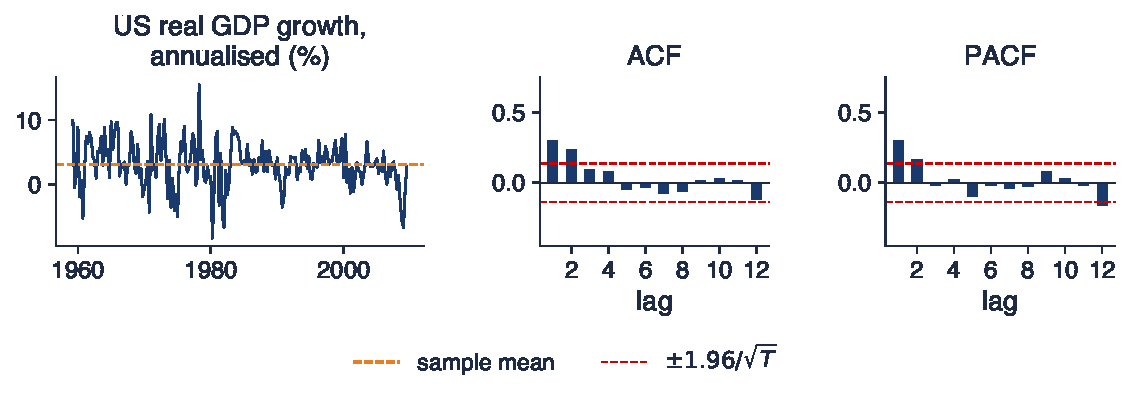
\includegraphics[width=0.96\textwidth,height=0.30\textheight,keepaspectratio]{ch2_sem_b1.pdf}
\end{center}
\vspace{-2mm}
\begin{center}
\scriptsize
\begin{tabular}{lrrrrr}
\toprule
 & WN & AR(1) & AR(2) & MA(2) & ARMA(1,1) \\
\midrule
AIC & 1084{,}56 & 1066{,}98 & \textbf{1063{,}70} & 1065{,}59 & 1065{,}02 \\
BIC & 1091{,}17 & \textbf{1076{,}91} & 1076{,}93 & 1078{,}83 & 1078{,}25 \\
\bottomrule
\end{tabular}
\end{center}
\begin{itemize}
    \item $T = 202$, ACF $0{,}30$; $0{,}24$; $0{,}09$ și PACF $0{,}30$; $0{,}16$; $-0{,}02$ (banda $\pm 0{,}14$): AR(1) sau AR(2)
    \item BIC: AR(1), $\hat\mu = 3{,}12$, $\hat\phi = 0{,}306$ (0{,}060); AIC: AR(2), $\hat\phi_2 = 0{,}163$ (0{,}062); valorile BIC diferă cu 0,02
    \item Reziduurile AR(1): $Q^*(8) = 11{,}08$ cu 7 grade de libertate, p = 0{,}135; Jarque--Bera 16{,}0, p $<$\,0{,}001
    \item Interpretare: timpul de înjumătățire $\ln 0{,}5/\ln 0{,}306 = 0{,}59$ trimestre: șocurile de creștere sînt de scurtă durată; persistența se află în nivelul producției, nu în ritmul de creștere
\end{itemize}\quantlet{TSA\_ch2\_seminar}{\qlurl{TSA_ch2_seminar}}
\end{frame}

\begin{frame}{B2: creșterea PIB-ului real al României [Propus]}
\itemsize{\footnotesize}
\begin{itemize}
\item \textbf{Întrebarea}: are creșterea trimestrială a PIB-ului real al României vreo structură ARMA?
\item \textbf{Date}: Eurostat, volume înlănțuite, ajustate sezonier și pentru zilele lucrătoare, T1 2000--T2 2026; $y_t = 100\,\Delta\ln Y_t$; model: B1
\item \textbf{Cerințe}
\begin{enumerate}
    \item Repetați cei patru pași din B1 pentru $y_t$ (\texttt{ro\_gdp\_growth('qoq')}).
    \item Aplicați testul Ljung--Box $Q^*(8)$ seriei însăși.
    \item Repetați analiza fără cele patru trimestre din 2020 și comparați.
    \item Interpretare: de ce cea mai bună prognoză a creșterii din trimestrul următor este pur și simplu media?
\end{enumerate}
\item \textbf{Raportați}: graficul, un tabel cu zece valori ale criteriilor, testele și două fraze
\item Notebook: secțiunea B2
\end{itemize}
\end{frame}

\ifsolutions
\begin{frame}{B2: rezolvare [Propus]}
\itemsize{\scriptsize}
\begin{center}
\includegraphics[width=0.96\textwidth,height=0.30\textheight,keepaspectratio]{ch2_sem_b2.pdf}
\end{center}
\vspace{-2mm}
\begin{center}
\scriptsize
\begin{tabular}{lrrrrr}
\toprule
 & WN & AR(1) & AR(2) & MA(2) & ARMA(1,1) \\
\midrule
AIC & \textbf{496{,}15} & 498{,}04 & 497{,}24 & 497{,}17 & 498{,}94 \\
BIC & \textbf{501{,}48} & 506{,}03 & 507{,}89 & 507{,}83 & 509{,}59 \\
\bottomrule
\end{tabular}
\end{center}
\begin{itemize}
    \item $T = 106$, media 0{,}83\%, abaterea standard 2{,}48\%; ACF $-0{,}03$; $-0{,}16$; $-0{,}04$ (banda $\pm 0{,}19$); minimul $-10{,}2\%$ în T1 2009
    \item Ambele criterii aleg zgomotul alb; $Q^*(8) = 7{,}5$, p = 0{,}481; Jarque--Bera 147{,}4, p $<$\,0{,}001; fără 2020: p = 0{,}793, abaterea standard 2{,}27\%
    \item Interpretare: creșterea trimestrială trecută nu conține informație liniară despre trimestrul următor; prognoza este $\hat\mu = 0{,}83\%$ (eroarea standard 0{,}30); rata anuală din curs este un MA(3) pentru că însumează patru astfel de trimestre
\end{itemize}
\end{frame}
\fi

\begin{frame}{B3: randamentele zilnice ale BET [Rezolvat]}
\itemsize{\footnotesize}
\begin{itemize}
\item \textbf{Întrebarea}: este autocorelația de ordinul 1 a randamentelor BET utilă pentru prognoză?
\item \textbf{Date}: închiderile BET din 2000 (EODHD); $r_t = 100\,\Delta\ln P_t$, $T = 6\,670$, ultima zi 18 septembrie 2026
\item \textbf{Cerințe}
\begin{enumerate}
    \item Estimați un AR(1) prin verosimilitate maximă și raportați $\hat\phi$, eroarea standard, raportul $t$ și $R^2$.
    \item Testați reziduurile cu Ljung--Box $Q^*(10)$, cu 9 grade de libertate, și pătratele reziduurilor cu $Q^*(10)$.
    \item Calculați boltirea și statistica Jarque--Bera a reziduurilor.
    \item Prognozați randamentul de mîine cu intervalul de 95\%.
    \item Interpretare: este coeficientul AR(1) semnificativ statistic și este el util din punct de vedere economic?
\end{enumerate}
\item \textbf{Raportați}: șase valori, graficul, o prognoză cu intervalul ei și două fraze
\item Notebook: secțiunea B3
\end{itemize}
\end{frame}

\begin{frame}{B3: rezolvare [Rezolvat]}
\itemsize{\scriptsize}
\begin{center}
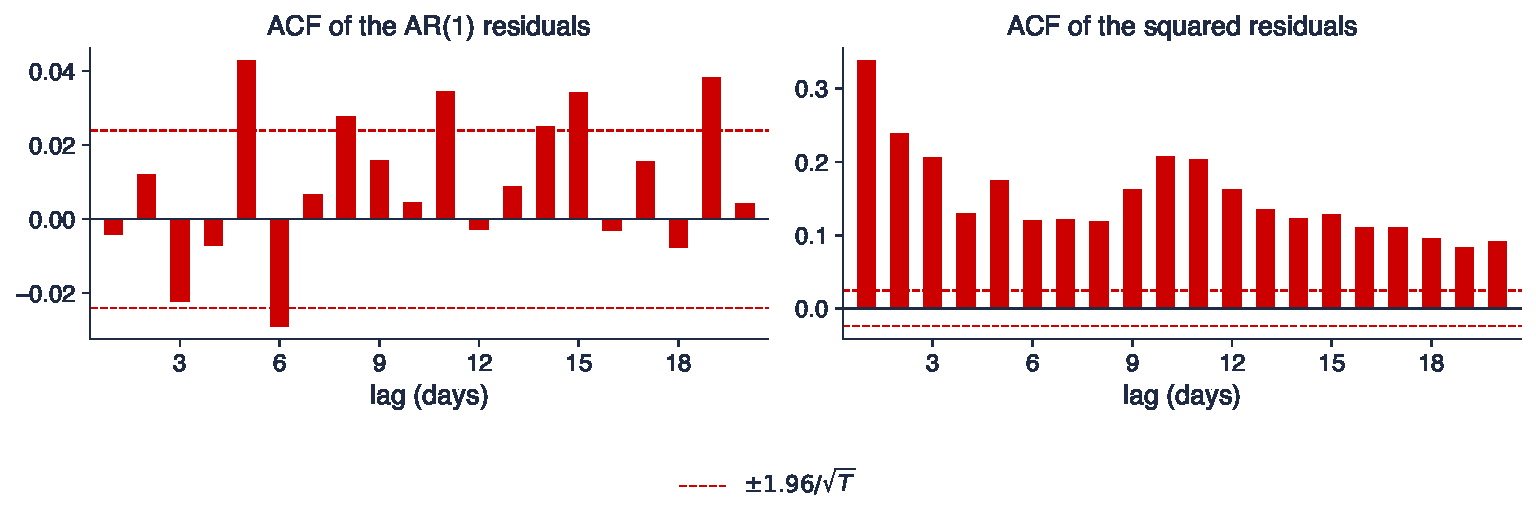
\includegraphics[width=0.96\textwidth,height=0.40\textheight,keepaspectratio]{ch2_sem_b3.pdf}
\end{center}
\vspace{-2mm}
\begin{itemize}
    \item $\hat\phi = 0{,}109$ (eroarea standard 0{,}0052), $t = 20{,}9$; $R^2 = 1{,}2\%$; $\hat\sigma = 1{,}390\%$
    \item Reziduurile: $Q^*(10) = 29{,}7$, p $<$\,0{,}001 (rămîne puțină corelație); pătratele: $Q^*(10) = 2496$; boltirea 14{,}0, Jarque--Bera 34128
    \item Ultimul randament $2{,}17\%$: prognoza $0{,}294\%$, intervalul de 95\% $[-2{,}43; 3{,}02]$ (construit cu distribuția Normală, prea îngust în cozi)
    \item Interpretare: foarte semnificativ, dar explică aproximativ 1\% din varianță, iar prognoza este foarte mică în raport cu intervalul; valoarea mare a lui $Q^*$ pentru pătrate trimite la modelele de volatilitate (\tsachlink{https://danpele.github.io/Time-Series-Analysis/RO/Cursuri/capitol5_volatilitate_conditionata_garch.pdf}{Capitolul 5})
\end{itemize}\quantlet{TSA\_ch2\_seminar}{\qlurl{TSA_ch2_seminar}}
\end{frame}

\begin{frame}{B4: randamentele zilnice EUR/RON [Propus]}
\itemsize{\footnotesize}
\begin{itemize}
\item \textbf{Întrebarea}: se comportă cursul EUR/RON ca BET?
\item \textbf{Date}: cursul de referință BNR din iulie 2005, $T = 5\,352$ randamente; model: B3
\item \textbf{Cerințe}
\begin{enumerate}
    \item Repetați cei patru pași din B3 (\texttt{b3\_returns('eurron')}).
    \item Comparați $\hat\phi$, $R^2$ și boltirea cu cele ale BET.
    \item Interpretare: de ce poate un curs de schimb administrat să aibă o autocorelație de ordinul 1 mai mare decît un indice bursier?
\end{enumerate}
\item \textbf{Raportați}: un tabel (două serii, cîte șase valori) și două fraze
\item Notebook: secțiunea B4
\end{itemize}
\end{frame}

\ifsolutions
\begin{frame}{B4: rezolvare [Propus]}
\itemsize{\scriptsize}
\begin{center}
\includegraphics[width=0.96\textwidth,height=0.34\textheight,keepaspectratio]{ch2_sem_b4.pdf}
\end{center}
\vspace{-2mm}
\begin{center}
\scriptsize
\begin{tabular}{lrrrrrr}
\toprule
 & $\hat\phi$ & $t$ & $R^2$ (\%) & $Q^*(10)$ & $Q^*_{sq}(10)$ & boltirea \\
\midrule
BET & $0{,}109$ & 20{,}9 & 1{,}2 & 29{,}7 & 2496 & 14{,}0 \\
EUR/RON & $0{,}170$ & 30{,}6 & 2{,}9 & 61{,}5 & 2351 & 17{,}0 \\
\bottomrule
\end{tabular}
\end{center}
\begin{itemize}
    \item EUR/RON: $\hat\phi$ și $R^2$ mai mari, corelație reziduală ($Q^*(10)$, p $<$\,0{,}001), cozi mai groase; prognoza $0{,}020\%$, intervalul $[-0{,}52; 0{,}56]$
    \item Interpretare: banca centrală netezește cursul, deci mișcările continuă una sau două zile; salturile mari și rare dau boltirea ridicată
\end{itemize}
\end{frame}
\fi


%=============================================================================
\section{Partea C: întrebări deschise și critica unui răspuns AI}
%=============================================================================

\begin{frame}{C1: bate un model AR prognozele simple ale inflației? [Propus]}
\itemsize{\footnotesize}
\begin{itemize}
\item \textbf{Întrebarea}: este un AR(2) mai bun decît media istorică și ultima valoare la prognoza inflației pe 12 luni din România, cu un an înainte?
\item \textbf{Date}: inflația IAPC din 2005 (Eurostat); origini de prognoză în fiecare lună începînd cu ianuarie 2015; modele: B1, A1
\item \textbf{Cerințe}
\begin{enumerate}
    \item La fiecare origine, estimați un AR(2) pe toate datele pînă în luna respectivă și prognozați cu 12 luni înainte.
    \item Calculați aceleași prognoze din media istorică și din ultima valoare observată.
    \item Comparați RMSE și MAE pentru cele trei metode, pe întreaga perioadă și înainte de iulie 2021.
    \item Interpretare: de ce eșuează toate cele trei metode în 2022?
\end{enumerate}
\item \textbf{Raportați}: un tabel cu RMSE și MAE, graficul și un plan de proiect
\item Notebook: secțiunea C1
\end{itemize}
\end{frame}

\ifsolutions
\begin{frame}{C1: analiză de referință [Propus]}
\itemsize{\scriptsize}
\begin{center}
\includegraphics[width=0.96\textwidth,height=0.36\textheight,keepaspectratio]{ch2_sem_c1.pdf}
\end{center}
\vspace{-2mm}
\begin{center}
\scriptsize
\begin{tabular}{lrrr}
\toprule
 & AR(2) & media & ultima valoare \\
\midrule
RMSE, total & 3{,}22 & 3{,}94 & 3{,}52 \\
MAE, total & 2{,}46 & 2{,}95 & 2{,}84 \\
RMSE, înainte de iulie 2021 & 1{,}97 & 3{,}16 & 2{,}10 \\
\bottomrule
\end{tabular}
\end{center}
\begin{itemize}
    \item 128 de prognoze pentru ianuarie 2016--august 2026; AR(2) are cele mai mici erori, dar avantajul față de ultima valoare este mic
    \item Interpretare: șocul energetic din 2022 a fost în afara istoriei seriei; un model univariat îl învață abia după aceea. Un proiect: adăugați un test formal (Diebold--Mariano), alte orizonturi și alte țări
\end{itemize}
\end{frame}
\fi

\begin{frame}{C2: verificați un răspuns AI [Propus]}
\itemsize{\scriptsize}
\begin{itemize}
    \item Un student a cerut unui asistent AI informații despre modelele ARMA din acest seminar. Răspunsul:
    \item \aiprompt{(a) Procesul X(t) = 0,6 X(t-1) + 0,5 X(t-2) + e(t) este staționar, deoarece ambii coeficienți sînt sub 1.}
    \item \aiprompt{(b) Un MA(1) cu theta = 2 nu este staționar, deoarece |theta| > 1.}
    \item \aiprompt{(c) Modelul AR(1) pentru randamentele BET are t = 21, deci randamentul de ieri explică cea mai mare parte a randamentului de azi.}
    \item \aiprompt{(d) Pentru reziduurile unui ARMA(1,1), statistica Ljung-Box Q(8) se compară cu distribuția hi-pătrat cu 8 grade de libertate.}
    \item \aiprompt{(e) Prognoza unui MA(2) cu trei pași înainte este egală cu media seriei.}
    \item \aiprompt{(f) Într-un AR(1), X(t) = c + phi X(t-1) + e(t), media seriei este c.}
    \item Cerințe
    \begin{itemize}
        \item 1. Pentru fiecare afirmație, precizați dacă este corectă; dacă nu, dați afirmația corectă și, unde se poate, valoarea corectă din notebook (secțiunea C2).
        \item 2. Raportați: o listă de șase verdicte, fiecare cu un rînd de justificare.
    \end{itemize}
\end{itemize}
\end{frame}

\ifsolutions
\begin{frame}{C2: rezolvare [Propus]}
\itemsize{\scriptsize}
\begin{itemize}
    \item (a) Greșit: $\phi_1 + \phi_2 = 1{,}1 > 1$; o rădăcină a lui $1 - 0{,}6z - 0{,}5z^2$ este în interiorul cercului: proces exploziv (exemplul C din curs)
    \item (b) Greșit: orice MA finit este staționar; $|\theta| > 1$ încalcă invertibilitatea, nu staționaritatea (A3)
    \item (c) Greșit: semnificativ nu înseamnă mare: $\hat\phi = 0{,}109$, $\hat\phi^2 \approx 1{,}2\%$ din varianță (B3)
    \item (d) Greșit: $8 - p - q = 6$ grade de libertate; cu 8 testul este prea indulgent (A6)
    \item (e) Corect: după $q = 2$ pași prognoza este $\mu$
    \item (f) Greșit: media este $c/(1 - \phi)$; $c$ este termenul liber (A1)
\end{itemize}\quantlet{TSA\_ch2\_seminar}{\qlurl{TSA_ch2_seminar}}
\end{frame}
\fi


%=============================================================================
\section{Încheiere}
%=============================================================================

\begin{frame}{Idei de reținut}
\itemsize{\small}
\begin{itemize}
    \item Staționaritatea se citește din rădăcinile lui $\phi(z)$, invertibilitatea din rădăcinile lui $\theta(z)$, niciodată din coeficienți luați separat
    \item Media unui model AR este $c/\phi(1)$, nu termenul liber $c$
    \item Box--Jenkins: ACF și PACF propun, AIC și BIC aleg, testele pe reziduuri verifică, prognozele se compară cu repere simple
    \item Testul Ljung--Box pentru reziduuri folosește $m - p - q$ grade de libertate
    \item Semnificativ statistic nu înseamnă mare din punct de vedere economic: comparați $\hat\phi^2$ cu intervalul de prognoză
\end{itemize}
\end{frame}

\begin{frame}{După seminar}
\itemsize{\small}
\begin{itemize}
    \item Cursul 2 deduce formulele de azi: rădăcini, invertibilitate, ponderi $\psi$, estimatori, criterii informaționale, intervale de prognoză, studiul Box--Jenkins pentru PIB-ul României
    \item Încercați cerințele [Propus] în notebook
    \item C1 poate deveni un proiect de echipă: prognoze ARMA ale inflației în România și în regiune, comparate cu repere simple
    \item Lectură: \refHP, cap.~3--4; \refFPP, cap.~9; \refBD, cap.~3
    \item \textbf{Seminarul are rol de exercițiu și nu se notează; rezolvările cerințelor [Propus] se discută la seminar}
\end{itemize}
\end{frame}


%=============================================================================
\section{Bibliografie}
%=============================================================================

\begin{frame}{Bibliografie}
\itemsize{\tiny}
\begin{itemize}
    \item Akaike, H. (1974). A new look at the statistical model identification. \textit{IEEE Transactions on Automatic Control}, 19(6), 716--723. \href{https://doi.org/10.1109/TAC.1974.1100705}{doi:10.1109/TAC.1974.1100705}
    \item Box, G. E. P., Jenkins, G. M., \& Reinsel, G. C. (2008). \textit{Time Series Analysis: Forecasting and Control} (4th ed.). Wiley. \href{https://doi.org/10.1002/9781118619193}{doi:10.1002/9781118619193}
    \item Box, G. E. P., \& Pierce, D. A. (1970). Distribution of residual autocorrelations in autoregressive-integrated moving average time series models. \textit{Journal of the American Statistical Association}, 65(332), 1509--1526. \href{https://doi.org/10.1080/01621459.1970.10481180}{doi:10.1080/01621459.1970.10481180}
    \item Brockwell, P. J., \& Davis, R. A. (2016). \textit{Introduction to Time Series and Forecasting} (3rd ed.). Springer. \href{https://doi.org/10.1007/978-3-319-29854-2}{doi:10.1007/978-3-319-29854-2}
    \item Huang, C., \& Petukhina, A. (2022). \textit{Applied Time Series Analysis and Forecasting with Python}. Springer. \href{https://doi.org/10.1007/978-3-031-13584-2}{doi:10.1007/978-3-031-13584-2}
    \item Hyndman, R. J., \& Athanasopoulos, G. (2021). \textit{Forecasting: Principles and Practice} (3rd ed.). OTexts. \href{https://otexts.com/fpp3/}{otexts.com/fpp3}
    \item Jarque, C. M., \& Bera, A. K. (1987). A test for normality of observations and regression residuals. \textit{International Statistical Review}, 55(2), 163--172. \href{https://doi.org/10.2307/1403192}{doi:10.2307/1403192}
    \item Ljung, G. M., \& Box, G. E. P. (1978). On a measure of lack of fit in time series models. \textit{Biometrika}, 65(2), 297--303. \href{https://doi.org/10.1093/biomet/65.2.297}{doi:10.1093/biomet/65.2.297}
    \item Schwarz, G. (1978). Estimating the dimension of a model. \textit{The Annals of Statistics}, 6(2), 461--464. \href{https://doi.org/10.1214/aos/1176344136}{doi:10.1214/aos/1176344136}
\end{itemize}
\end{frame}

\end{document}
